\section{\content{電腦中的漢字}{电脑中的汉字}}\label{section:電腦中的漢字}
\content{進入現代以後,電腦成為了人們讀寫漢字的新媒介。如今資訊科技高度發達,許多人使用電腦來讀寫的時間已經遠遠超過了使用紙筆。媒介的改變當然會帶來讀寫方式的改變,於是人們設計數位字體以供顯示漢字,設計輸入法以供鍵入漢字。}{进入现代以后,电脑成为了人们读写汉字的新媒介。如今信息技术高度发达,许多人使用电脑来读写的时间已经远远超过了使用纸笔。媒介的改变当然会带来读写方式的改变,于是人们设计数码字體以供显示汉字,设计输入法以供键入汉字。}\par
\content{在本節,筆者將簡要介紹一些電腦漢字相關的知識。如果你對「亂碼」的來歷感到好奇,對中文輸入法的選擇有些困惑,或者是想了解印刷體與手寫體的區別,那就一定不要錯過本節的內容。}{在本节,笔者将简要介绍一些电脑汉字相关的知识。如果你对“乱码”的来历感到好奇,对中文输入法的选择有些困惑,或是是想了解印刷体与手写体的区别,那就一定不要错过本节的内容。}\par
\subsection{\content{中文輸入法}{中文输入法}}\label{subsection:中文輸入法}
\content{我們一般所說的「輸入法」可以分解成兩個層次的概念:\textbf{輸入法方案}與\textbf{輸入法程式}。很多人在比較輸入法時,經常把方案之間的比較與程式之間的比較相混淆,從而引起很多不必要的爭執。筆者認為自己有義務對這些概念加以解釋。}{我们一般所说的“输入法”可以分解成两个层次的概念:\textbf{输入法方案}与\textbf{输入法程序}。很多人在比较输入法时,经常把方案之间的比较与程式之间的比较相混淆,从而引起很多不必要的争执。笔者认为自己有义务对这些概念加以解释。}\par
\subsubsection{\content{輪入法方案}{输入法方案}}
\content{輸入法方案關乎於每個字的編碼。在倉頡碼中「輸」的編碼是\charcode{十十人一弓},對應到鍵盤上就是\charcode{jjomn};在漢語全拼中的編碼則是\charcode{shu},對應鍵盤上的\charcode{shu}。}{输入法方案关乎于每个字的编码。在仓颉码中“输”的编码是\charcode{大手人一弓},对应到键盘上就是\charcode{kqomn};在汉语全拼中的编码则是\charcode{shu},对应键盘上的\charcode{shu}。}\par
\content{一種最死板的輸入法方案是,直接把所有漢字亂序編碼。我們只要強記這些編碼,就可以在鍵盤上打出任何一個想要的字。Unicode輸入法便是如此,我們只需敲下「輸」的編碼\charcode{8f38}就可以得到這個字。}{一种最死板的输入方案是,直接把所有汉字乱序编码。我们只要强记这些编码,就可以在键盘上打出任何一个想要的字。Unicode便入法便是如此,我们只需敲下“输”的编码\charcode{8f93}就可以得到这个字。}\par
\content{這類編碼的缺陷顯而易見:各個漢字與其編碼之間沒有任何邏輯關聯。為了正常使用,人們必須強行記住每個字的編碼,而這樣巨大的記憶量將使人望而卻步。所以人們當然更傾向於把漢字與其編碼關聯起來,用「推導」代替不必要的「記憶」。這種邏輯關聯的本質就是直接分析一個字的音、形、義,由此推算出編碼。分析字義並不可行,所以主流的中文輸入法要麼是基於字音的\textbf{音碼輸入法},要麼是基於字形的\textbf{形碼輸入法}。}{这类编码的缺陷显而易见:各个汉字与其编码之间没有任何逻辑关联。为了正常使用,人们必须强行记住每个字的编码,而这样巨大的记忆量将使人望而却步。所以人们当然更倾向于反汉字与其编码关联起来,用“推导”代替不必要的“记忆”。这种逻辑关联的本质就是直接分析一个字的音、形、义,由此推算出编码。分析字义并不可行,所以主流的中文输入法要么是基于字音的\textbf{音码输入法},要么是基于字形的\textbf{形码输入法}。}\par
\content{音碼輸入法的拆字思路比較簡單:根據漢語拼音、注音符號或粵語拼音等,把一個字的讀音轉換成編碼。「輸」的粵語拼音是\boxpinyin{syu},對應到粵拼方案上就是\charcode{syu};拼音是\boxpinyin{shu},對應到自然碼雙拼方案上就是\charcode{uu}\footnote{在自然碼雙拼中,聲母\boxpinyin{sh}對應到\charcode{u}鍵。此方案還提供了字形輔助碼,但那不是必需部分。};注音是\boxzhuyin{ㄕㄨ},對應到大千式注音方案上就是\charcode{gj}。對於受過良好拼音/注音教育的人來說,字音輸入法的優點就是上手簡單,易學易用——無論你是否會寫,只要你知道它的讀音,你就知道它在拼音/注音中如何拆,然後你只需要在鍵盤上敲下對應的鍵\footnote{在台灣,許多電腦鍵盤不止印有英數字母,還印有注音符號甚至倉頡、大易字根,所以在鍵盤上就可以直接找到注音符號的位置。}就可以了。}{音码输入法的拆字思路比较简单:根据汉语拼音、注音符号或粵语拼音等,把一个字的读音转换成编码。“输”的粵语拼音是\boxpinyin{syu},对应到粵拼方案上就是\charcode{syu};拼音是\boxpinyin{shu},对应到自然码双拼方案上就是\charcode{uu}\footnote{在自然码双拼中,声母\boxpinyin{sh}对应到\charcode{u}键。此方案还提供了字形辅助码,但那不是必需部分。};注音是“ㄕㄨ”,对应到大千式注音方案上就是\charcode{gj}。对于受过良好拼音/注音教育的人来说,字音输入法的优点就是上手简单,易学易用——无论你是否会写,只要你知道它的读音,你就知道它在拼音/注音中如何拆,然后你只需要在键盘上敲下对应的键\footnote{在台湾,许多电脑键盘不止印有英数字母,还印有注音符号甚至仓颉、大易字根,所以在键盘上就可以直接找到注音符号的位置。}就可以了。}\par
\begin{wrapfigure}{O}{.38\textwidth}
	\centering
	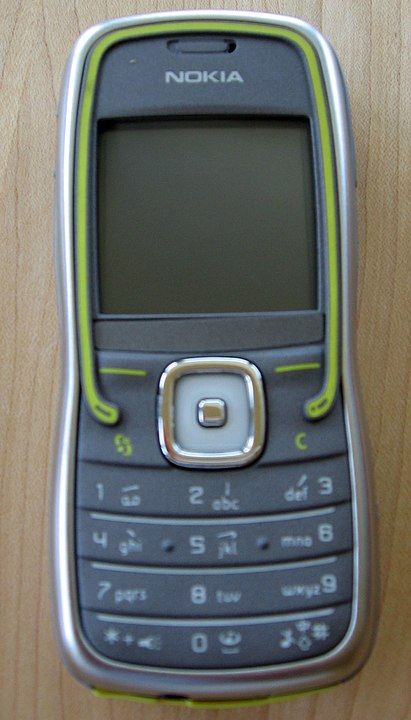
\includegraphics[width=.38\textwidth]{Nokia_5500.jpg}
	\caption{\content{一款諾基亞傳統型手機}{一款诺基亚传统型手机}}
	\label{figure:一款諾基亞傳統型手機}
	\footnotesize{\color{darkgray}\content{鍵盤1-5對應有筆順鍵}{键盘1-5对应有笔顺键}}
\end{wrapfigure}
\content{音碼輸入法往往都基於既有的拼音/注音方案,在拆字思路上大同小異;但形碼輸入法就五花八門了。最細碎的筆畫輸入法把每個字的筆畫都拆開來,分成「橫竪撇點折」五類,每一筆都是一碼,那麼「輸」字要敲上足足16碼。因為編碼過長,輸入效率很低,所以幾乎沒有人再使用了,只在傳統型手機的九鍵鍵盤中還有保留(\cref*{figure:一款諾基亞傳統型手機})。}{音码输入法往往都基于既有的拼音/注音方案,在拆字思路上大同小异;但形码输入法就五花八门了。最细碎的笔画输入法把每个字的笔画都拆开来,分成“横竖撇点折”五类,每一笔者是一码,那么“输”字要敲上足足13码。因为编码过长,输入效率很低,所以几乎没有人再使用了,只在传统型手机的九键键盘中还有保留(\cref*{figure:一款諾基亞傳統型手機})。}\par
\content{很多字的成分非常複雜,一筆一畫寫出來不現實,所以我們需要限制每個字的編碼長度,只取其中的若干成分,作為\textbf{字根}。一個字的編碼將根據它的字根及結構來確定。四角號碼便是如此。它規定一個字必須編四碼\footnote{這里不考慮附角。如果考慮附角的話,應是五碼。},在編碼時分別看這個字左上角、右上角、左下角、右下角的字根形狀,再把字根轉換為對應的數字。還以「輸」字為例,它的左上角和左下角是連起來的一個「插」畫,所以左上角取\charcode{5},左下角用\charcode{0}代替;右上角的「人」是「八」畫,取\charcode{8};右下角的「亅」是「垂」畫,取\charcode{2}。所以「輸」字的四角號碼為\charcode{5802}。}{很多字的成分非常复杂,一笔一画写出来不现实,所以我们需要限制每个字的编码长度,只取其中的若干成分,作为\textbf{字根}。一个字的编码将根据它的字根及结构来确定。四角号码便是如此。它规定一个字必须编四码\footnote{这里不考虑附角。如果考虑附角的话,应是五码。},在编码时分别看这个字左上角、右上角、左下角、右下角的字根形状,再把字根转换为对应的数字。还以“输”字为例,这个字左上角的“𠂇”是“叉”画,取\charcode{4};右上角的“人”是“八”画,取\charcode{8};左下角的“𰀁”是“插”画,取\charcode{5};右下角的“亅”是“垂”画,取\charcode{2}。所以“输”字的四角号码为\charcode{4852}。}\par
\content{四角號碼發明於20世紀初。當時四角號碼並非用於打字,而是用於「檢字」\footnote{最典型的檢字就是根據字形查字典。很多人只會用部首檢字法,即:先根據部首的筆畫數量找到部首所在頁,再根據剩餘的筆畫數量從同部首的字中找到目標字。這種檢字方法容易學,但效率偏低,因為既要確定部首,又要數出筆畫數量,還需要在很多字中找到目標字。用四角號碼來檢字就方便很多。}。後來有人把四角號碼加以改良,製成縱橫輸入法。縱橫碼的思路也是根據漢字四角的成分來取碼。}{四角号码发明于20世纪初。当时的四角号码并非用于打字,而是用于“检字”\footnote{最典型的检字就是根据字形查字典。很多人只会用部首检字法,即:先根据部首的笔画数量找到部首所在页,再根据剩余的笔画数量从同部首的字中找到目标字。这种检字方法容易学,但效率偏低,因为既要确这部首,又要数出笔画数量,还需要在很多字中找到目标字。用四角号码来检字就方便很多。}。后来有人把四角号码加以改良,制成纵横输入法。纵横码的思路也是根据汉字四角的成分来取码。}\par
\content{筆順、四角和縱橫所需的編碼鍵較少,所以在九鍵鍵盤或電腦小鍵盤上仍有用武之地;但在大鍵盤上,我們完全可以把字根分得更細緻。大易輸入法和行列40輸入法使用了40個鍵;行列30輸入法使用了30個鍵;鄭碼、徐碼、嘸蝦米使用了26個鍵;倉頡輸入法\footnote{不含六代倉頡輸入法(或曰「蒼頡輸入法」)。}、五筆字體輸入法使用了25個鍵\footnote{倉頡的\charcode{重}和五筆的\charcode{z}都不是必需的,不計入。}。}{笔顺、四角和纵横所需的编码键较少,所在在九键键盘或电脑小键盘上仍有用武之地;但在大键盘上,我们完全可以把字根分得更细致。大易输入法和行列40输入法使用了40个键;行列30输入法使用了30个键;郑码、呒虾米输入法使和了26个键;仓颉输入法\footnote{不含六代仓颉输入法(或曰“苍颉输入法”)。}、五笔字體输入法使用了25个键\footnote{仓颉的\charcode{重}和五笔的\charcode{z}都不是必需的,不计入。}。}\par
\content{不同的形碼輸入法可能採用完全不同的字根體系、拆字方式和編碼方式。但無論如何,只要給定一套規則,我們就可以對任何一個字進行編碼。這就是「輸入法方案」所關注的問題。}{不同的形码输入法可能采用完全不同的字根体系,拆字方式和编码方式。但无论如何,只要给定一套规则,我们就可以对任何一个字进行编码。这就是“输入法方案”所关注的问题。}\par
\subsubsection{\content{輸入法程式}{输入法程序}}
\content{筆者對形碼輸入法了解較多,常聽到有人比較形碼輸入法時給出這樣的說法:}{笔者对形码输入法了解较多,常听到有人比较形码输入法时给出这样的说法:}
\begin{itemize}
	\item \content{甲輸入法沒有容錯碼,有些字因為某些原因有多種拆碼方式,但人們只能按其中一種編碼來鍵入,換另一種合理的編碼卻打不出想要的字;乙輸入法卻有容錯碼。所以乙輸入法更好。}{甲输入法没有容错码,有些字因为某些原因有多种拆码方式,但人们只能按其中一种编码来键入,换另一种合理的编码却打不出想要的字;乙输入法却有容错码。所以乙输入法更好。}
	\item \content{甲輸入法只支援打簡體字,不支援打繁體字(或者正相反);乙輸入法既能打繁體字,又能打簡體字,還能打日本漢字、假名、諺文等。所以乙輸入法更好。}{甲输入法只支持打简体字,不支持打繁体字(或者正相反);乙输入法既能打繁体字,又能打简体字,还能打日本汉字、假名、谚文等。所以乙输入法更好。}
	\item \content{甲輸入法只能打些常用字,遇到生僻字就打不出來了;乙輸入法卻能打很多生僻字。所以乙輸入法更好。}{甲输入法只能打些常用字,遇到生僻字就打不出来了;乙输入法却能打很多生僻字。所以乙输入法更好。}
	\item ……
\end{itemize}
\content{這類說法有一個共性:它們本應是輸入法程式層面的比較,而不是輸入法方案層面的比較。然而人們常常把這些程式層面的問題延伸到方案上去,變成了「五筆打不了繁體字,來學倉頡」或者「倉頡不支援異體字,來學某某」云云,這是一種不自知的偷換概念。}{这类说法有一个共性:它们本应是输入法程式层面的比较,而不是输入法方案层面的比较。然而人们常常把这些程式层面的问题延伸到方案上去,变成了“五笔打不了繁体字,来学仓颉”或者“仓颉不支持异体字,来学某某”云云,这是一种不自知的偷换概念。}\par
\begin{wrapfigure}{O}{.3\textwidth}
	\centering
	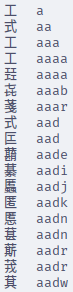
\includegraphics[width=.15\textwidth]{五筆碼表部分.png}
	\caption{\content{一份YAML格式的五筆碼表(部分)}{一份YAML格式的五笔码表(部分)}}
	\label{figure:一份YAML格式的五筆碼表}
\end{wrapfigure}
\content{電腦不會自動地根據輸入法方案所述的規則,對每個字進行編碼;這項工作必須由人來完成。輸入法程式的設計者需要按照輸入法方案的規則,把每個字的編碼確定下來,編成一張\textbf{碼表}。}{电脑不会自动地根据输入法方案所述的规则,对每个字进行编码;这项工作必须由人来完成。输入法程序的设计者需要按照输入法方案的规则,把每个字的编码确定下来,编成一张\textbf{码表}。}\par
\content{有了碼表之後,電腦才能根據你輸入的編碼,找到這個編碼對應的字——也就是你想要的字。以\cref*{figure:一份YAML格式的五筆碼表}為例,輸入五筆編碼\charcode{aadn}能得到「慝葚」兩個項,我們可以選字輸入。但是如果碼表中沒有「慝」呢?我們用\charcode{aadn}自然打不出「慝」字;候選項中只有「葚」這一個字。同樣的道理,\textbf{如果一個碼表中只有簡體字,我們就打不出繁體字;如果一個碼表中只有常用字,我們就打不出生僻字。}有人說「五筆輸入法打不出繁體字」,那是因為他所用的輸入法「程式」所帶碼表中沒有繁體字,並不是五筆輸入法這個「方案」本身不支援繁體字(實際上五筆方案是支援繁體字的,它有繁體字字根)。}{有了码表之后,电脑才能根据你输入的编码,找到这个编码对应的字——也就是你想要的字。以\cref*{figure:一份YAML格式的五筆碼表}为例,输入五笔编码\charcode{aadn}能得到“慝葚”两个项,我们可以选字输入。但是如果码表中没有“慝”呢?我们用\charcode{aadn}自然打不出“慝”字;候选项中只有“葚”这一个字。同样的道理,\textbf{如果一个码表中只有简体字,我们就打不出繁体字;如果一个码表中只有常用字,我们就打不出生僻字。}有人说“五笔输入法打不出繁体字”,那是因为他所用的输入法“程序”所带码表中没有繁体字,并不是五笔输入法这个“方案”本身不支持繁体字(实际上五笔方案是支持繁体字的,它有繁体字字根)。}\par
\content{容錯碼的處理也屬於程式方面的問題。就以「黃」字來說,它的港標寫法和台標寫法有著細微的不同:港標寫法是「{\hk 黃}」,中間是「由」字形;台標寫法則是「黃」,中間是「田」字形。如果某套倉頡輸入法碼表只考慮了港標字形而把此字編碼成\charcode{廿一中金}的話,台標用戶就會感到困惑:明明按「黃」字形拆成\charcode{廿一田金},卻怎麼也找不到這個字。一款做得細緻的輸入法程式會充分考慮到這種異寫造成的編碼不唯一問題,並採用有容錯碼的碼表;而有些輸入法程式就沒有考慮過這些問題。但是無論如何,\textbf{這個鍋應該交給輸入法程式來背,不該讓輸入法方案來背。}}{容错码的处理也属于程序方面的问题。就以“黄”字来说,它的港标写法与台标写法有着细微的不同:港标写法是“{\hk 黃}”,中间是“由”字形;台标写法则是“{\tw 黃}”,中间是“田”字形。如果某套仓颉输入法码表只考虑了港标字形而把此字编码成\charcode{廿一中金}的话,台标用户就会感到困惑:明明按“{\tw 黃}”字形拆成\charcode{廿一田金},却怎么也找不到这个字。一款做得细致的输入法程序会充分考虑到这种异写造成的编码不唯一问题,并采用有容错码的码表;而有些输入法程序就没有考虑过这些问题。但是无论如何,\textbf{这个锅应该交给输入法程序来背,不该让输入法方案来背。}}\par
\content{還有很多個性化的功能也是程式相關的,與方案無關。有些形碼輸入法支援形碼與拼音混輸,那是因為程式設計者把兩套碼表結合起來了;有些輸入法支援動態詞頻,那是因為輸入法程式有一套統計和計算方法;有些五筆輸入法允許四碼唯一自動上屏,以及第五碼頂字上屏,那是程式設計者為了提高輸入效率而做的功能優化;有些形碼輸入法支持用拼音反查編碼,這是輸入法程式的附加功能;有些音碼輸入法支援模糊音\footnote{多數方言系統與普通話系統所含聲韻母不同,於是說慣了方言的人在學習普通話拼音時有可能分不清某些聲韻母,比如\bopin{ㄋ}{n}與\bopin{ㄌ}{l},\bopin{ㄣ}{en}與\bopin{ㄥ}{eng}等。很多拼音輸入法為了照顧這些群體,會設計出模糊音功能。這樣一來,敲\bopin{ㄕˋ}{\pinyin{shi4}}可以出「四」,敲\bopin{ㄙˊ}{\pinyin{si2}}也可以出「十」。},這也是程式設計者應該考慮的工作……凡此種種,不一而足。可是有些人在比較輸入法「方案」時卻有意或無意地把「程式」的優劣也拿來當作參考,那就不公平了!}{还有很多个性化的功能也是程序相关的,与方案无关。有些形码输入法支持形码与拼音混输,那是因为程序设计者把两套码表结合起来了;有些输入法支持动态词频,那是因为输入法程序有一套统计和计算方法;有些五笔输入法允许四码唯一自动上屏,以及第五码顶字上屏,那是程序设计者为了提高输入效率而做的功能优化;有些形码输入法支持用拼音反查编码,这是输入法程序的附加功能;有些音码输入法支持模糊音\footnote{多数方言系统与普通话系统所含声韵母不同,于是说惯了方言的人在学习普通话拼音时有可能分不清某些声韵母,比如\bopin{ㄋ}{n}与\bopin{ㄌ}{l},\bopin{ㄣ}{en}与\bopin{ㄥ}{eng}等。很多拼音输入法为了照顾这些群体,会设计出模糊音功能。这样一来,敲\bopin{ㄕˋ}{\pinyin{shi4}}可以出“四”,敲\bopin{ㄙˊ}{\pinyin{si2}}也可以出“十”。},这也是程序设计者应该考虑的工作……凡此种种,不一而足。可是有些人在比较输入法“方案”时却有意无意地把“程序”的优劣也拿来当作参考,那就不公平了!}\par
\content{在輸入法領域,提出一套輸入法方案的人一般都要做一個輸入法程式並釋出,否則光有方案沒有程式,就是紙上談兵。其他人也可能根據這套方案,自行設計輸入法程式;甚至改良原有方案,做成更適合某些受眾的新方案,再做成輸入法程式。Rime輪入引擎更是提供了高度個性化的選擇,使用戶能夠自定義輸入法的功能、碼表——通俗點說,用戶可以利用Rime自己設計輸入法程式,不用擔心市面上的輸入法沒有自己想要的功能。所以時至今日,我們不應該再拿「輸入法程式」層面的指標去作比較了,因為「你有什麼功能,我也可以有;哪怕現在沒有,我也可以做給你看」。但作為輸入法之核心的「方案」,才能真正決定一個字「應該怎麼拆、應該怎麼編碼」,這才是我們比較輸入法時真正應該思考的部分。}{在输入法领域,提出一套输入法方案的人一般都要做一个输入法程序并发布,否则光有方案没有程序,就是纸上谈兵。其他人也可能根据这套方案,自行设计输入法程序;甚至改良原有方案,做成更适合某些受众的新方案,再做成输入法程序。Rime输入引擎更是提供了高度个性化的选择,使用户能够自定义输入法的功能、码表——通俗点说,用户可以利用Rime自己设计输入法程序,不用担心市面上的输入法没有自己想要的功能。所以时至今日,我们不应该再拿“输入法程序”层面的指标去作比较了,因为“你有什么功能,我也可以有;哪怕现在没有,我也可以做给你看”。但作为输入法之核心的“方案”,才能真正决定一个字“应该怎么拆、应该怎么编码”,这才是我们比较输入法时真正应该思考的部分。}\par
\subsubsection{\content{音碼、形碼與音形碼}{音码、形码与音形码}}
\content{前面說過,主流輸入法基本分為音碼輸入法與形碼輸入法。當然也有二者結合的音形碼輸入法。}{前面说过,主流输入法基本分为音码输入法与形码输入法。当然也有二者结合的音形码输入法。}\par
\content{有些音形碼方案的設計初衷在於降低音碼方案的\textbf{重碼率}——漢字中的同音字太多,如果純用音碼的話,會有很多字編碼相同\footnote{筆者簡單統計了一下,自己所用的拼音碼表中有797個\bopin{ㄧ}{yi}音的字,351個\bopin{ㄕ}{shi}音的字和301個\bopin{ㄨ}{wu}音的字。保守估計,非生僻字至少佔到10\%,這就意味著同一編碼下可能有數十個常見字。},我們不得不翻好幾頁來選詞,這樣就極大影響了輸入效率。雙拼方案可以有效地減少編碼長度,把每一字固定在2碼長,但對降低重碼率沒有幫助。既然依賴字音不能降低重碼,那麼還是要從字形出發,把同音字從編碼上分開來。}{有些音形码方案的设计初衷在于降低音码方案的\textbf{重码率}——汉字中的同音字太多,如果纯用音码的话,会有很多字编码相同\footnote{笔者简单统计了一下,自己所用的拼音码表中有797个\bopin{ㄧ}{yi}音的字,351个\bopin{ㄕ}{shi}音的字和301个\bopin{ㄨ}{wu}音的字。保守估计,非生僻字至少占到10\%,这就意味着同一编码下可能有数十个常见字。},我们不得不翻好几页来选词,这样就极大影响了输入效率。双拼方案可以有效地减少编码长度,把每一字固定在2码长,但对降低重码率没有帮助。既然依赖字音不能降低重码,那么还是要从字形出发,把同音字从编码上分开来。}\par
\content{小鶴音形就是這樣一種音形碼方案。它規定每個字最多編四碼,前兩碼為雙拼碼(音碼),後兩碼為形碼。比如「衣」和「佚」字,它們的雙拼都是\charcode{yi};但若加上後兩碼的形碼,就分別變成\charcode{yiwy}和\charcode{yiru},這樣就減少了重碼。自然碼雙拼方案也採用了形碼作為輔碼。雖然這些輸入方案都是音形碼,但用戶完全可以無視「形」的部分,純粹將其當成音碼輸入法來用。}{小鹤音形就是这样一种音形码方案。它规定每个字最多编四码,前两码为双拼码(音码),后两码为形码。比如“衣”和“佚”字,它们的双拼都是\charcode{yi};但若加上后两码的形码,就分别变成\charcode{yiwy}和\charcode{yiru},这样就减少了重码。自然码双拼方案也采用了形码作为辅码。虽然这些输入方案都是音形码,但用户完全可以无视“形”的部分,纯粹将其当成音码输入法来用。}\par
\content{有些音形碼輸入法則必須嚴格包含音形兩部分,二筆音形輸入法便是如此。它規定,一個字最多編四碼,第一碼取拼音首字母,後三碼按筆順取筆畫\footnote{就形碼的處理來說,二筆音形要比原始的筆畫輸入法高明些;但它的缺陷還是有很多,後文再談。感興趣的讀者可以自行查詢二筆輸入法的相關資料。}。以「輸」字為例,它的拼音是\boxpinyin{\pinyin{shu1}},所以第一碼取\charcode{s}。後三碼根據字形及結構取\charcode{jrk},這裡就不詳細解釋了。}{有些音形码输入法则必须严格包含音形两部分,二笔音形输入法便是如此。它规定,一个字最多编四码,第一码取拼音首字母,后三码按笔顺取笔画\footnote{就形码的处理来说,二笔音形要比原始的笔画输入法高明些;但它的缺陷还是有很多,后文再谈。感兴趣的读者可以自行查询二笔输入法的相关资料。}。以“输”字为例,它的拼音是\boxpinyin{\pinyin{shu1}},所以第一码取\charcode{s}。后三码根据字形及结构取\charcode{;rk},这里就不详细解释了。}\par
\content{不少人對嚴格的音形碼持批評態度,因為用戶在鍵入時必須要既知其音,又知其形。「齷齪」比較難寫,許多人不記得字形,但用音碼輸入法就可以很方便地打出來;「轡」「蠹」二字比較生僻,許多人不知道讀音,但用形碼輸入法也可以打出來\footnote{這種情況一般出現於需要依字形檢字的場合,或者抄錄內容的場合。總之,使用者知道或能看到字形,但不知道讀音。若是音、形全都不知道,那就根本沒辦法,不在討論之列。}。然而若是用了音形碼呢?以上兩類字全都不會打。所以僅就這個方面來說,音形碼的缺陷比單純的音碼、形碼都要大。}{不少人对严格的音形码持批评态度,因为用户在键入时必须要既知其音,又知其形。“龌龊”二字比较难写,许多人不记得字形,但用音码输入法就可以很方便地打出来;“辔”“蠹”二字比较生僻,许多人不知道读音,但用形码输入法也可以打出来\footnote{这种情况一般出现于需要依字形检字的场合,或者抄录内容的场合。总之,使用者知道或能看到字形,但不知道读音。若是音、形全都不知道,那就根本没办法,不在讨论之列。}。然而若是用了音形码呢?以上两类字全都不会打。所以仅就这个方面来说,音形码的缺陷比单纯的音码、形码都要大。}\par
\content{而自然碼、小鶴這些雙拼方案就比較靈活。它們雖然是音形碼方案,但我們完全可以把它當作音碼方案來用,所以不知道字形也沒有什麼大礙(有不少用戶壓根不學輔碼部分,也一樣能用好雙拼)。}{而自然码、小鹤这些双拼方案就比较灵活。它们虽然是音形码方案,但我们完全可以把它当作音码方案来用,所以不知道字形也没有什么大碍(有不少用户压根不学辅码部分,也一样能用好双拼)。}\par
\content{音碼的重碼率問題是由音碼方案本身所決定的,無法避免。音形碼方案能在一定程度上降低重碼率,但是,一方面,它要求用戶兼知音形才能打出一個字來;另一方面,很多音形碼方案只能降低單字重碼率,而無法降低詞組重碼率——例如,雙拼方案在輸入詞組時,只取每字的音碼,不取輔碼。恐怕只有純形碼方案能做到比較低的重碼率了。}{音码的重码率问题是由音码方案本身所决定的,无法避免。音形码方案能在一定程度上降低重码率,但是,一方面,它要求用户兼知音形才能打出一个字来;另一方面,很多音形码方案只能降低单字重码率,而无法降低词组重码率——例如,双拼方案在输入词组时,只取每字的音码,不取辅码。恐怕只有纯形码方案能做到比较低的重码率了。}\par
\content{在中文輸入法發展的早期,形碼曾因為低重碼、快速、適合盲打而受到許多人(尤其是專業人士)的青睞。後來音碼輸入法在「程式」層面做了諸多改進,比如智慧選字、動態詞頻、雲端詞庫、整句輸入、長句聯想等功能,使得輸入法程式越來越易用。這樣一來,雖然重碼率沒有下降,但「概率最高的選項」往往能排在最靠前的位置,於是用戶就可以少受翻頁選詞之苦了。}{在中文输入法发展的早期,形码曾因为低重码、快速、适合盲打而受到许多人(尤其是专业人士)的表睐。后来音码输入法在“程序”层面做了诸多改进,比如智能选字、动态词频、云端词库、整句输入、长句联想等功能,使得输tyif程序越来越易用。这样一来,虽然重码率没有下降,但“概率最高的选项”往往能排在最靠前的位置,于是用㧀不可以少受翻页选词之苦了。}\par
\content{對於音碼輸入法\footnote{尤指有智慧功能的音碼輸入法。現在市面上流行的大多數輸入法程式都或多或少配備這些功能了。}來說,\textbf{以詞為單位,甚至以短語/整句為單位來輸入,能夠有效提高輸入法的效率}。這點很好理解:如果別人用語音說了單獨一個字,你幾乎猜不到他說的到底是哪個字,因為同音字太多了;如果他說了一個詞,你大概能猜到幾個可能性,但未必能完全確定;而如果他說了一個短語或者一句話,那你幾乎就可以猜到每個字都是什麼了。這是因為,上下文為我們判斷文字提供了資訊量。對於智慧型輸入法來說,也是如此。}{对于音码输入法\footnote{尤指有智能功能的音码输入法。现在市面上流行的大多数输入法程序都或多或少配备这些功能了。}来说,\textbf{以词为单位,甚至以短语/整句为单位来输入,能够有效提高输入法的效率}。这点很好理解:如果别人用语音说了单独一个字,你几乎猜不到他说的到底是哪个字,因为同音字太多了;如果他说了一个词,你大概能猜到几个可能性,但未必能完全确定;而如果他说了一个短语或者一句话,那你几乎就可以猜到每个字都是什么了。这是因为,上下文为我们判断文字提供了信息量。对于智能输入法来说,也是如此。}\par
\content{而形碼輸入法則相反,\textbf{以詞組為單位來輸入,未必能提高輸入法的效率}。不僅如此,動態詞頻等智慧功能還可能成為輸入法使用過程中的跘腳石。形碼方案基本上無法區分一段編碼有幾個字\footnote{對於音碼編碼來說就很容易。大部分漢字都是有聲母的,所以在處理編碼時,從聲母處斷開就可以解決九成以上的斷字問題。},於是對於一個四碼長的編碼來說,單字、二字詞、三字詞等都會出現在候選項中。本來,單字的重碼率並不高;但加上詞組之後,候選項就變多了,重碼率也就增加了。換句話說,用單字時重碼少到幾乎可以盲打,但用單字/詞組混合時重碼卻多到很難支援我們盲打了。動態詞頻也有類似的問題:如果某字時而在第一位,時而在第二位,那麼我們就不能依靠盲打的記憶慣性來敲出此字了。}{而形码输入法则相反,\textbf{以词组为单位来输入,未必能提高输入法的效率}。不仅如此,动态词频等智能功能还可能成为输入法使用过程中的跘脚石。形码方案基本上无法区分一段编码有几个字\footnote{对于音码编码来说就很容易。大部分汉字都是有声母的,所以在处理编码时,从声母处断开就可以解决九成以上的断字问题。},于是对于一个四码长的编码来说,单字、二字词、三字词等都会出现在候选项中。本来,单字的重码率并不高;但加上词组之后,候选项就变多了,重码率也就增加了。换句话说,用单字时重码少到几乎可以盲打,但用单字/词组混合时重码却多到很难支持我们盲打了。动态词频也有类似的问题:如果某字时而在第一位,时而在第二位,那么我们就不能依靠盲打的记忆惯性来敲出此字了。}\par
\content{然而輸入時用單字不用詞組,無疑會減慢打字的速度——這也是形碼輸入法面臨的一個尷尬之處。面對這些問題,大概每個用戶都會做出自己的選擇吧!}{然而输入时用单字不用词组,无疑会减慢打字的速度——这也是形码输入法面临的一个尴尬之处。面对这些问题,大概每个用户都会做出自己的选择吧!}\par
\subsubsection{\content{選擇形碼輸入法的參考指標}{选择形码輸入法的参考指标}}
\content{市面上的形碼輸入法方案種類繁多。不少新人挑花了眼,也沒有選出最中意的一款。筆者自認為對形碼輸入法比較了解,可以向讀者介紹一下如何比較形碼方案\footnote{音碼方案的邏輯一般要比形碼方案簡單,所以下文所述的指標基本可以包含音碼的評價標準。想要選擇音碼輸入法的用戶也可以參考這些內容。}。不過請注意,筆者雖然會舉一些輸入法作為比較用的例子,但並不打算向讀者「推薦」任何一款輸入法;讀者應當根據這些資訊,自行判斷哪款方案最合你心意。}{市面上的形码输入法方案种类繁多。不少新人挑花了眼,也没有选出最中意的一款。笔者自认为对形码输入法比较子解,可以向读者介绍一下如何比较形码方案\footnote{音码方案的逻辑一般要比形码方案简单,所以下文所述的指标基本可以包含音码的评价标准。想要选择音三输入法的用户也可以参考这些内容。}。不过请注意,笔者虽然会举一些输入法作为比较用的例子,但并不打算向读者“推荐”任何一款输入法;读者应当根据这些信息,自行判断哪款方案最合你心意。}\par
\content{從用戶的角度來說,用形碼輸入法打單字可以分成兩個過程:先是「\textbf{拆字根}」,按輸入法規則,從一個字中拆出若干個字根;再是「\textbf{找按鍵}」,找到每個字根分別位於哪些鍵,依次按下。因此,\textbf{拆字如何進行},\textbf{字根如何歸位},就是評價形碼輸入法的核心指標。當然,除此之外還有零零散散的其它指標。}{从用户的角度来说,用形码输入法打单字可以分成两个过程:先是“\textbf{拆字根}”,按输入法规则,从一个字中拆出若干个字根;再是“\textbf{找按键}”,找到每个字根分别位于哪些键,依次按下。因此,\textbf{拆字如何进行},\textbf{字根如何归位},就是评价形码输入法的核心指标。当然,除此之外还有零零散散的其它指标。}\par
\subsubsubsection{\content{作業系統的支援情況}{操作系统的支持情况}}
\content{我們使用中文輸入法,總要依托於某些輸入法程式。很多中文作業系統都會自帶一些輸入法程式,比如Windows的微軟輸入法,支援簡體中文的拼音、五筆86和繁體中文的注音、倉頡、大易、行列等\footnote{順便一提,很多常見輸入法,如嘸蝦米,它們並沒有內置到Windows中,其實是因為輸入法的所有者並未公開版權,也並未授權給微軟使用。}。只要你會其中的一種輸入法,換任何一台Windows電腦都可以輕鬆打字。但如果你學習了別的輸入法,那就必須安裝相應的輸入法程式才能使用。}{我们使用中文输入法,总要依托于某些输入法程序。很多中文操作系统都会自带一些输入法程序,比如Windows的微软输入法,支持简体中文的拼音、五笔86和繁体中文的注音、仓颉、大易、行列等\footnote{顺便一提,很多常见输入法,如呒虾米,它们并没有内置到Windows中,其实是因为输入法的所有者并示公开版权,也并未授权给微软使用。}。只要你会其中的一种输入法,换任何一台Windows电脑都可以轻松打字。但如果你学习了别的输入法,那就必须安装相应的输入法程序才能使用。}\par
\content{當然了,裝個輸入法其實也沒什麼費勁的,畢竟是一項一勞永逸的工作。但是,假如你要臨時使用其它的電腦呢?如果你不會那些自帶輸入法的話,難道也要臨時裝一個嗎——更何況有些商業軟體每安裝在一台電腦上都要花一份錢。}{当然了,装个输入法其实也没什么费劲的,毕竟是一项一劳永逸的工作。但是,假如你要临时使用其它的电脑呢?如果你不会那些自带输入法的话,难道也要临时装一个吗——更何况有些商业软件每安装在一台电脑上都要花一份钱。}\par
\content{除了Windows之外,MacOS和Linux也都有一些自帶輸入法,大致也還是拼音、五筆、注音、倉頡這些常見類型。然而個別小眾輸入法卻僅僅照顧了Windows用戶——他們只開發了能用於Windows的程式,卻無視了其它作業系統用戶的需求。有些人學了這個方案,到頭來卻根本不能在別的作業系統中使用,因為沒有這樣的輸入法程式。}{除了Windows之外,MacOS和Linux也都有一些自带输入法,大致也还是拼音、五笔、注音、仓颉这些常见类型。然而个别小众输入法却仅仅照顾了Windows用户——他们只开发了能用于Windows的程序,却无视了其它操作系统用户的需求。有些人学了这个方案,到头来却根本不能在别的操作系统中使用,因为没有这样的输入法程序。}\par
\content{手機的情況與電腦稍有不同,因為手機輸入法往往依賴軟鍵盤,而不像電腦輸入那樣常用硬鍵盤。軟鍵盤不受硬體的限制,可以更靈活地排布按鍵,所以很多電腦上不容易做/不適合做的方案(比如拼音9鍵和拼音14鍵)可以很方便地做到手機中。讀者也不該總是被硬鍵盤局限住。如果覺得某款手機輸入方案比較好,就大膽嘗試吧!你完全可以在電腦和手機上分別使用不同的輸入方案。}{手机的情况与电脑稍有不同,因为手机输入法往往依赖软键盘,而不像电脑输入那样常用硬键盘。软键盘不受硬件的限制,可以更灵活地排布按键,所以很多电脑上不容易做/不适合做的方案(比如拼音9键和拼音14键)可以很方便地做到手机中。读者也不该总是被硬键盘局限往。如果学得某款手机输入方案比较好,就大胆尝试吧!你完全可以在电脑和手机上分别使用不同的输入方案。}\par
\subsubsubsection{\content{碼長規則}{码长規則}}
\content{除了筆畫輸入法這種有多少畫就編多少碼的方案以外,絕大多數輸入法都會規定編碼的長度。四角、縱橫輸入法是定長四碼,無論哪個字都要編成四碼;三角輸入法則是定長六碼。五筆、鄭碼、嘸蝦米等方案是最長四碼,每個字最多編四碼;倉頡則是最長五碼。大易有三個版本,原版大易又叫「大易四碼」,規定最長四碼;大易三碼規定最長三碼,大易二碼規定最長二碼\footnote{所幸大易可以用40個鍵,這樣能讓編碼相對分散些;如果像四角那樣只有10個鍵,那麼最長二碼的設計簡直能帶來重碼災難。}。}{除了笔画输入法这种有多少画就编多少码的方案以外,绝大多数输入法都会规定编码的长度。四角、纵横输入法是定长四码,无论哪个字都要编成四码;三角输入法则是定长六码。五笔、郑码、呒虾米等方案是最长四码,每个字最多编四码;仓颉则是最长五码。大易有三个版本,原版大易又叫“大易四码”,规定最长四码;大易三码规定最长三码,大易二码规定最长二码\footnote{所幸大易可以用40个键,这样能让编码相对分散些;如果像四角那样只有10个键,那么最长二码的设计简直能带来重码灾难。}。}\par
\content{碼長短的好處是輸入效率高;但如果碼長限制得太短,就會產生大量的重碼,反而將降低輸入效率。以倉頡為例,這是常見方案中唯一規定最長五碼的方案。倉頡長期以來都是重碼率最低的方案\footnote{倉頡方案在設計之初就是為了兼容所有漢字(以至設計中文作業系統,詳見\href{https://zh.wikipedia.org/zh-tw/倉頡系統}{倉頡系統-維基百科}),而重碼問題一直是倉頡設計者關注的重點。},直到近年來才被徐碼等新興輸入法所趕超\footnote{相關數據請參考\href{https://terryhung.pixnet.net/blog/post/24986976}{老話一句:不要學嘸蝦米,學倉頡!——泰瑞的世界|痞客邦},以及\href{https://yuhao.forfudan.com/docs/statistics.html}{常見輸入法測評數據|宇浩輸入法網站}。};但因為最長五碼以及沒有簡碼(見後文)的緣故,倉頡並不是輸入最快的方案。}{码长短的好处是输入效率高;但如果码长限制得太短,就会产生大量的重码,反而将降低输入效率。以仓颉为例,这是常见方案中唯一规定最长五码的方案。仓颉长期以来都是重码率最低的方案\footnote{仓颉方案在设计之初就是为了兼容所有汉字(以至设计中文操作系统,详见\href{https://zh.wikipedia.org/zh-cn/倉頡系統}{仓颉系统-维基百科}),而重码问题一直是仓颉设计者关注的重点。},直到近年来才被徐码等新兴输入法所赶超\footnote{相关数据请参考\href{https://terryhung.pixnet.net/blog/post/24986976}{老话一句:不要学呒虾米,学仓颉!——泰瑞的世界|痞客邦},以及\href{https://yuhao.forfudan.com/docs/statistics.html}{常见输入法测评数据|宇浩输入法网站}。};但因为最长五码以及没有简码(见后文)的缘故,仓颉并不是输入最快的方案。}\par
\subsubsubsection{\content{字根的細碎程度}{字根的细碎程度}}
\content{很多形碼輸入法使用比較大塊的字根,比如五筆當中「車」就是一個字根,編碼為\charcode{l}。於是我們打「輸」字時想到字形中整塊的「車」字根就知道它是\charcode{l},不需要進一步分析其字形了。但若是使用二筆、行列的話,它們沒有「車」這樣大塊的字根,所以還要進一步分析筆畫才能得出其編碼,這樣就不夠直觀,不易學習。}{很多形码输入法使用比较大块的字根,比如五笔当中“车”就是一个字根,编码为\charcode{l}。于是我们打“输”字时想到字形中整块的“车”字根就知道它是\charcode{l},不需要进一步分析其字形了。但若是使用二笔、行列的话,它们没有“车”这么大块的字根,所以还要是一步分析笔画才能得出其编码,这样就不够直观,不易学习。}\par
\content{但大塊字根也有其問題。首先,漢字偏旁十分豐富,若是全用大塊的字根,那麼字根的總量一定非常多,於是使用者就需要記憶大量字根的編碼。而且,字根量大必然導致不同字根歸入同一鍵区,於是這些字根就無法區分,從而引發重碼,比如大易把「耳」「身」兩字根都歸入\charcode{p}鍵使得「職」與其異體字「軄」形成一組重碼字。}{但大块字根也有其问题。首先,汉字偏旁十分丰富,若是全用大块的字根,那么字根的总量一定非常多,于是使用者就需要记忆大量字根的编码。而且,字根量大必然导致不同字根归入同一键区,于是这些字根就无法区分,从而引发重码,比如大易把“耳”“身”两字根都归入\charcode{p}键使得“職”(“职”字繁体)与其异体字“軄”形成一组重码字。}\par
\subsubsubsection{\content{字根的單編碼與雙編碼}{字根的单编码与双编码}}
\content{較古的字形輸入法一般都是簡單地把多個字根歸入同一鍵中。這樣就會造成許多字根無法分辨,進而帶來重碼問題。如果能夠把字根的編碼分得更精細,或許就可以解決這一問題。}{较古的字形输入法一般都是简单地把多个字根归入同一键中。这样就会造成许多字根无法分辨,进而带来重码问题。如果能够把字根的编码分得更精细,或许就可以解决这一问题。}\par
\content{鄭碼是最早嘗試「雙編碼字根」的輸入方案。後來的徐碼、虎碼、宇浩等輸入方案也都採用了雙編碼。這些雙編碼的規則大同小異,基本上都可以如此詮譯:}{郑码是最早尝试“双编码字根”的输入方案。后来的徐码、虎码、宇浩等输入方案也都采用了双编码。这些双编码的规则大同小异,基本上都可以如此诠释:}\par
\begin{enumerate}
	\item \content{當不同字根歸在同一「區」時,選擇一個構字頻率較高的字根,作為「主根」\footnote{有些雙編碼方案不設主根。無妨,這不影響本文的核心内容。}。主根的編碼就是這個區的編碼,叫做「區碼」或「大碼」。}{当不同字根归在同一“区”时,选择一个构字频率较高的字根,作为“主根”\footnote{有些双编码方案不设主根。无妨,这不影响文本的核心内容。}。主根的编码就是这个区的编码,叫做“区码”或“大码”。}
	\item \content{位於同一區的其它字根都是副根\footnote{鄭碼中有「第二主根」的說法。但從本質上講,第二主根的地位及處理方式與副根無異,而與「第一主根」不同。其它方案如徐碼等也不存在「第二主根」這種說法,所以筆者認為這是一個多餘的概念。}。副根由「區碼」和「位碼」(又叫「小碼」)構成,位碼能夠用來進一步區分同一區的字根。}{位于同一区的其它字根都是副根\footnote{郑码中有“第二主根”的说法。但从本质上讲,第二主根的地位及处理方式与副根无异,而与“第一主根”不同。其它方案如徐码等也不存在“第二主根”这种说法,所以笔者认为这是一个多余的概念。}。副根由“区码”和“位码”(又叫“小码”)构成,位码能够用来进一步区分同一区的字根。}
\end{enumerate}
\content{舉個例子:鄭碼「月」「几」「犭」「殳」「九」這五個字根都在\charcode{Q}區,其中「月」是主根(用大寫字母表示),編碼為\charcode{Q}。其餘四個副根都有自己的位碼(用小寫字母表示),分別編碼為「几\charcode{Qd}」「犭\charcode{Qm}」「殳\charcode{Qx}」「九\charcode{Qy}」。}{举个例子:郑码“月”“几”“犭”“殳”“九”这五个字根都在\charcode{Q}区。其中“月”是主根(用大写字母表示),编码为\charcode{Q}。其余四个副根都有自己的位码(用小写字母表示),分别编码为“几\charcode{Qd}”“犭\charcode{Qm}”“殳\charcode{Qx}”“九\charcode{Qy}”。}\par
\content{鄭碼使用大塊字根。若是每個字根都用單編碼,必然造成很多重碼。舉個例子,如果「木」編碼為\charcode{F}而「甘」和「其」都編碼成\charcode{E},那麼「柑」和「棋」的編碼都是\charcode{fe},無法區分。但在鄭碼中「甘」有雙編碼\charcode{Eb},「其」有雙編碼\charcode{Ec},那麼「柑」「棋」就分別是\charcode{feb}\charcode{fec},這樣便不重碼了!}{郑码使用大块字根。或是每个字根都用单编码,必然造成很多重码。举个例子,如果“木”编码为\charcode{F}而“甘”和“其”都编码成\charcode{E},那么“柑”和“棋”的编码都是\charcode{fe},无法区分。但在郑码中“甘”有双编码\charcode{Eb},“其”有双编码\charcode{Ec},那么“柑”“棋”就分别是\charcode{feb}\charcode{fec},这样便不重码了!}\par
\content{多數雙編碼方案都限制了單字碼長,規定最長四碼。為了保證較低的重碼率,這些方案通常都有稍顯複雜的取碼規則。但是,規則上複雜一點並不會導致輸入法很難學!真正使得輸入法難學的,其實是那些規則以外的「特例」與「潜規則」。而在規則方面,鄭碼等方案設計得相當規範,並不難學。如果一定要說雙編碼方案有什麼難學之處的話——筆者覺得記憶區位碼要比較麻煩,畢竟大部分字根都是雙編碼的,肯定要比單編碼難記。}{多数双编码方案都限制了单字码长,规定最长四码。为了保证较低的重码率,这些方案通常都有稍显复杂的取码规则。但是,规则上复杂一点并不会导致输入法很难学!真正使得输入法难学的,其实是那些规则以外的“特例”与“潜规则”。而在规则方面,郑码等方案设计得相当规范,并不难学。如果一定要说双编码方案有什么难学之处的话——笔者学得记忆区位码要比较麻烦,毕竟大部分字根都是双编码的,肯定要比单编码难记。}\par
\subsubsubsection{\content{字根歸位的有理性}{字根归位的有理性}}
\content{考慮完了字根性質的問題,我們再來看看字根歸位的問題,也就是:一個字根放到哪一區(雙編碼字根還要考慮放到哪一位),又對應鍵盤上的哪一鍵。}{考虑完了字根性质的问题,我们再来看看字根归位的问题,也就是:一个字根放到哪一区(双编码字根还要考虑放到哪一位),又对应键盘上的哪一键。}\par
\content{許多初學者苦於記憶字根和鍵盤的對應關係,便去尋求「記誦口訣」。學過86版五筆的人大概對這樣的句子很是耳熟:}{许多初学者苦于记忆字根和键盘的对应关系,便去寻求“记诵口诀”。学过86版五笔的人大概对这样的句子很是耳熟:}
\begin{boxquote}{86版五筆字根口訣}
	\content{
		王旁青頭戔(兼)五一,土士二干十寸雨,大犬三(羊)古石厂,\\
		木丁西,工戈草頭右框七……
	}{
		王旁青头戋(兼)五一,土士二干十寸雨,大犬三(羊)古石厂,\\
		木丁西,工戈草头右框七……
	}
\end{boxquote}
\content{幾乎每個形碼輸入法都有一些官方或民間的字根口訣,但並非所有口訣都是有價值的!就拿上述這個口訣來說,它能告訴你「某一鍵有哪些字根」;但在真正用輸入法打字時,我們需要知道的是「某一字根在哪個鍵」。如果不記得某個字根在哪一鍵的話,我們就必須從口訣第一句開始背,直到找到為止,效率太低。}{几乎每个形码输入法都有一些官方或民间的字根口诀,但并非所有口诀都是有价值的!就拿上述这个口诀来说,它能告诉你“某一键有哪些字根”;但在真正用输入法打字时,我们需要知道的是“某一字根在哪个键”。如果不记得某个字根在哪一键的话,我们就必须从口诀第一句开始背,直到找到为止,效率太低。}\par
\content{多數形碼輸入法在排布字根時並非胡亂排序,而是有一定的理據。比如說,形似的字根會歸入同一區(如倉頡);寫法符合一定筆順規則的字根會歸入同一區(如五筆);還有些方案會以形、音、義及鍵盤上的字母來綜合歸位(如嘸蝦米)。理順了輸入方案的歸位邏輯之後,我們可以直接「分析」一個字根應該如何編碼,完全不需要依靠什麼口訣(筆者學習五筆和倉頡時,從未利用所謂的口訣來助記)。}{多数形码输入法在排布字根时并非胡乱排序,而是有一定的理据。比如说,形似的字根会归入同一区(如仓颉);写法符合一定笔顺规则的字根会归入同一区(如五笔);还有些方案会以形、音、义及键盘上的字母来综合归位(如呒虾米)。理顺了输入方案的归位逻辑之后,我们可以直接“分析”一个字根应该如何编码,完全不需要依靠什么口诀(笔者学习五笔和仓颉时,从未利用所谓的口诀来助记)。}\par
\content{既然歸位邏輯對於初學者而言如此重要,那麼一套良好的、規範的歸位邏輯自然能夠讓用戶事半功倍地學成輸入法方案。相反,若是出現了大量規則以外的「特例」,那就無疑會增加學習的難度。比如,86版五筆將「力」字根歸入\charcode{l}是因為拼音的聲母為\bopin{ㄌ}{l},這是完全脫離五筆方案一般字根歸位原則的。我們需要把這些字根當成特例去記,這就是「無理碼」。}{既然归位逻辑对于初学者而言如此重要,那么一套良好的、规范的归位逻辑自然能够让用户事半功倍地学成输入法方案。相反,若是出现了大量规则以外的“特例”,那就无疑会增加学习的难度。比如,86版五笔将“力”字根归入\charcode{l}是因为拼音的声母为\bopin{ㄌ}{l},这是完全脱离五笔方案一般字根归位原则的。我们需要把这些字根当成特例去记,这就是“无理码”。}\par
\content{使用無理碼可能是因為很現實的原因,比如降低重碼率。如果百分百地按照既定規則去拆,總會有些構字性質相似的字根分布在同一區,進而造成重碼;所以就為這類字根指定了別的編碼。但過多的無理碼只會破壞字根歸位邏輯,加重學習時的記憶負擔。}{使用无理码可能是因为很现实的原因,比如降低重码率。如果百分百地按照既定规则去拆,总会有些构字性质相似的字根分布在同一区,进而造成重码;所以就为这类字根指定了别的编码。但过多的无理码只会破坏字根的归位逻辑,加重学习时的记忆负担。}\par
\content{還有一種情況是,字根歸位邏輯本身就混亂不堪。嘸蝦米輸入法把字根與英文字母關聯起來(這並非不可),至於關聯的方式就五花八門了——形似者如「亼\charcode{A}」,取拼音聲母者如「不\charcode{B}」,取字義者如「車\charcode{C}」(居然還是用英文意思car來解釋的!)。「云」字根因為形如注音字母\bopin{ㄊ}{t}而取碼\charcode{T},這簡直是要求人既想到注音又想到拼音。「言」字則是因為它的簡化偏旁「讠」形似\charcode{i}而取碼\charcode{I},這要讓不會簡化字的人怎麼辦?「冎」按官方說法是取音,但有幾人能知它讀作\bopin{ㄍㄨㄚˇ}{\pinyin{gua3}}?可是「冎」字根在\charcode{Q}鍵又是怎麼回事?}{还有一种情况是,字根归位逻辑本身就混乱不堪。呒虾米输入法把字根与英文字母关联起来(这并非不可),至于关联的方式就五花八门了——形似者如“亼\charcode{A}”,取拼音声母者如“不\charcode{B}”,取字义者如“車\charcode{C}”(居然还是用英文意思car来解释的!)。“云”字根因为形如注音字母\bopin{ㄊ}{t}而取码\charcode{T},这简直是要求人既想到注音又想到拼音。“言”字则是因为它的简化偏旁“讠”形似\charcode{i}而取码\charcode{I},这要让只会繁体字不会简化字的人怎么办?“冎”按官方说法是取音,但有几人能知它读作\bopin{ㄍㄨㄚˇ}{\pinyin{gua3}}?可是“冎”字根在\charcode{Q}键又是怎么回事?}\par
\content{最麻煩的問題還是出現在使用時。試問讀者,你能猜出「佳」「气」「彡」這三個字根要怎麼編碼嗎?是取其形、其音,還是其義?取音時要取聲母,還是韻母,還是介音,還是諧音?沒學過嘸蝦米的人們,大概是想破腦袋也想不出來的。答案是,「佳」字取「Very good」的含義,編碼為\charcode{V};「气」字取它的諧音,編碼為\charcode{K};「彡」取其形,編碼為\charcode{M}。大概嘸蝦米字根的歸位邏輯源自於天馬行空的想象,而用戶就要絞盡腦汁地跟上設計者的思路,最後卻還是難逃大量的死記硬背。}{最麻烦的问题还是出现在使用时。试问读者,你能猜出“佳”“气”“彡”这三个字根要怎么编码吗?是取其形、其音还是其义?取音时要取母,还是韵母,还是介音,还是谐音?没学过呒虾米的人,大概是想破脑袋也想不出来的。答案是,“佳”字取“Very good”的含义,编码为\charcode{V};“气”字取它的谐音,编码为\charcode{K};“彡”取其形,编码为\charcode{M}。大概呒虾米字根的归拉逻辑源自于天马行空的想象,而用户就要绞尽脑汁地跟上设计者的思路,最后却还是难逃大量的死记硬背。}\par
\content{反觀倉頡輸入法,它的字根歸位邏輯就合理得多——只考慮字形,而不是形音義相揉雜。並且倉頡輸入法沒有無理碼,每個字根為何歸入某鍵,都能說得清道理\footnote{可以參考\href{https://zh.wikibooks.org/wiki/倉頡輸入法/輔助字形}{倉頡輸入法/輔助字形-維基教科書}。}。於是二者相較,高下立判。}{反观仓颉输入法,它的字根归位逻辑就合理得多——只考虑字形,而不是形音义相杂揉。并且仓颉输入法没有无理码,每个字根为何归入某键,都能说得清道理\footnote{可以参考\href{https://zh.wikibooks.org/wiki/倉頡輸入法/輔助字形}{仓颉输入法/输助字形-维基教科书}。}。于是二者相较,高下立判。}\par
\subsubsubsection{\content{拆字是否斷筆畫、是否按筆順}{拆字是否断笔画、是否按笔顺}}
\content{說完了字根,我們再來看拆字的問題。很多初學縱橫、倉頡等輸入方案的人會對這些方案的拆字思路很不習慣。它們不像手寫漢字或五筆、大易等輸入法那樣取完整的筆畫,而是經常在同一筆處斷成兩三段,每段分別歸入不同的字根。以\cref*{figure:縱橫、倉頡輸入法斷筆拆字示例}為例,「司」字的「𠃌」畫在縱橫中被拆成了三個字根,「串」的「丨」畫在倉頡中被斷成二段,併入上下兩個字根。}{说完了字根,我们再来看拆字的问题。很多初学纵横、仓颉等输入方案的人会对这些方案拆字思路很不习惯。它们不像手写汉字或五笔、大易等输入法那样取完整的笔画,而是经常在同一笔处断成两三段,每段分别归入不同的字根。以\cref*{figure:縱橫、倉頡輸入法斷筆拆字示例}为例,“司”字的“𠃌”画在纵横中被拆成了三个字根,“串”的“丨”画在仓颉中被断成二段,并入上下两个字根。}\par
\begin{figure}[H]
	\centering
	\begin{subcaptionblock}{.45\textwidth}
		\centering
		\begin{tikzpicture}
			\node at(0,0){\fontsize{60}{0}\textit{司}};
			\node(左上)at\content{(-.3,.7)}{(-.35,.75)}[draw,red,ellipse,minimum width=15]{};
			\node(右上)at\content{(.45,.7)}{(.4,.75)}[draw,blue,ellipse,minimum width=16,minimum height=16]{};
			\node(左下)at\content{(-.25,-.15)}{(-.35,-.15)}[draw,olive,ellipse,minimum width=25,minimum height=20]{};
			\node(右下)at\content{(.35,-.65)}{(.3,-.65)}[draw,orange,ellipse,minimum width=15,minimum height=15]{};
			\node(左上根)at(-1.5,1.5)[red]{\content{橫}{横}};
			\node(右上根)at(1.5,1.5)[blue]{\content{角}{角}};
			\node(左下根)at(-1.5,-1.5)[olive]{\content{方塊}{方块}};
			\node(右下根)at(1.5,-1.5)[orange]{\content{左勾}{左勾}};
			\draw[red](左上根.south west)--(左上根.south east)--(左上);
			\draw[blue](右上根.south east)--(右上根.south west)--(右上);
			\draw[olive](左下根.north west)--(左下根.north east)--(左下);
			\draw[orange](右下根.north east)--(右下根.north west)--(右下);
		\end{tikzpicture}
		\caption{\content{縱橫輸入法拆「司」}{纵横输入法拆“司”}}
	\end{subcaptionblock}%
	\begin{subcaptionblock}{.45\textwidth}
		\centering
		\begin{tikzpicture}
			\node at(0,0){\fontsize{60}{0}\textit{串}};
			\node(一)at\content{(-.05,.5)}{(0,.55)}[draw,red,ellipse,minimum width=40,minimum height=20]{};
			\node(二)at\content{(0,-.3)}{(.05,-.25)}[draw,blue,ellipse,minimum width=45,minimum height=25]{};
			\node(一根)at(-1.5,1.5)[red]{\content{中}{中}};
			\node(二根)at(1.5,-1.5)[blue]{\content{中}{中}};
			\draw[red](一根.south west)--(一根.south east)--(一);
			\draw[blue](二根.north east)--(二根.north west)--(二);
		\end{tikzpicture}
		\caption{\content{倉頡輸入法拆「串」}{仓颉输入法拆“串”}}
	\end{subcaptionblock}%
	\caption{\content{縱橫、倉頡輸入法斷筆拆字示例}{纵横、仓颉输入法断笔拆字示例}}
	\label{figure:縱橫、倉頡輸入法斷筆拆字示例}
\end{figure}
\content{不少人因為斷筆拆字的緣故,對這類輸入法頗有微詞。持這樣觀點的人一般有三種理由:}{不少人因为断笔拆字的缘故,对这类输入法颇有微词。持这样观点的人一般有三种理由:}\par
\content{\textit{斷筆拆字不合字理,像「串」那樣拆成兩個「中」根本說不通。}其實,在漢字演變過程中筆畫的拆分與合併都很常見。若是字字都要依字理去拆,那就不該拿今天的漢字來拆,倒是該用古字形了——大可不必。甚至有些字中的筆畫自始至終都是連成一筆寫的,比如「里」,而它的字理卻是「田土」\footnote{「里」字的古義是居所。},不是「日土」或「甲二」。總之,形碼輸入法拆字時根本就不該考慮字理字義,否則就要亂套了。}{\textit{断笔拆字不合字理,像“串”那样拆成两个“中”根本说不通。}其实,在汉字演变过程中笔画的拆分与合并都很常见。若是字字都要依字理去拆,那就不该拿今天的汉字来拆,倒是该用古字形了——大可不必。甚至有些字中的笔画自始至终都是连成一笔写的,比如“里”,而它的字理却是“田土”\footnote{“里”字的古义是居所。},不是“日土”或“甲二”。总之,形码输入法拆字时根本就不该考虑字理字义,否则就要乱套了。}\par
\content{\textit{斷筆拆字違背了平常的書寫習慣,不容易學習。}的確,對於腦中只有文字筆畫卻無完整字形的人來說,斷筆拆字會很痛苦,筆者不推薦學習;但是,如果你還能記得字形的話,其實斷筆拆字並沒有多難學,因為從視覺上分析字形是非常直觀的。}{\textit{断笔拆字违背了平常的书写习惯,不容易学习。}的确,对于脑中中有文字笔画却无完整字形的人来说,断笔拆字会很痛苦,笔者不推荐学习;但是,如果你还能记得字形的话,其实断笔拆字并没有多难学,因为从视觉上分析字形是非常直观的。}\par
\begin{wrapfigure}{O}{.2\textwidth}
	\centering
	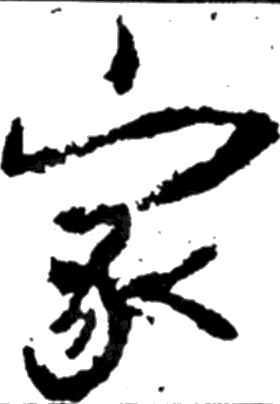
\includegraphics[width=.1\textwidth]{行書/家-李邕}
	\caption{\content{唐李邕行書「家」}{唐李邕行书“家”}}
	\label{figure:唐李邕行書「家」}
\end{wrapfigure}
\content{\textit{若是用慣這樣斷筆拆字的輸入法,恐怕連寫字都會出問題。}這樣想的人大概既不懂變通,又不清楚筆畫與筆順形成的過程,只是把現有的筆畫和筆順當作強制性規範來遵守。正常人為求書寫的順畅和方便,都會有意無意地把空間距離較近的筆畫連筆書寫,例如行書中常見「家」的「冖」部分連成一筆,甚至「丆」部分也會連成一筆,見\cref*{figure:唐李邕行書「家」}。而像「司」「串」那樣顯然是一筆寫下來的筆畫,又怎會因為輸入法中「斷筆」就真的被分成兩筆、三筆來書寫呢?}{\textit{若是用惯这样断笔拆字的输入法,恐怕连写字都会出问题。}这样想的人大概既不懂变通,又不清楚笔画与笔顺形成的过程,只是把现有的笔画和笔顺当作强制性规范来遵守。正常人为求书写的顺畅和方便,都会有意无意地把空间距离较近的笔画连笔书写,例如行书中常见“家”的“冖”部分连成一笔,甚至“丆”部分也会连成一笔,见\cref*{figure:唐李邕行書「家」}。而像“司”“串”那样显然是一笔写下来的笔画,又怎会因为输入法中“断笔”就真的被分成两笔、三笔来书写呢?}\par
\content{另一個同類問題是筆順。很多形碼輸入法在拆字時都要按照筆順的順序來取碼,而有些輸入法則不是。縱橫碼是固定地按照四個角的字形來取碼,不存在筆順問題;倉頡碼則是按照一定方向從視覺上把文字剪開,完全不按筆順來取碼。}{另一个同类问题是笔顺。很多形码输入法在拆字时都要按照笔顺的顺序来取码,而有些输入不则不是。纵横码是固定地按照四个角的字形来取码,不存在笔顺问题;仓颉码则是按照一定方向从视觉上把文字剪开,完全不按笔顺来取码。}\par
\content{按筆順拆字的好處是取碼方式容易學習,大家平常怎麼寫字,就按什麼順序來取字根。但問題恰恰出在這裡:很多字的筆順是因人而異的!}{按笔顺拆字的好处是取码方式容易学习。大家平常怎么写字,就按什么顺序来取字根。但问题恰恰出在这里:很多字的笔顺是因人而异的!}\par
\begin{wrapfigure}{O}{.23\textwidth}
	\centering
	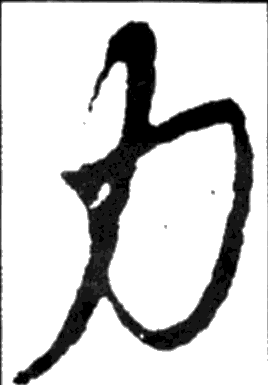
\includegraphics[width=.1\textwidth]{行書/力-王羲之}
	\caption{\content{晉王羲之行書「力」}{晋王羲之行书“力”}}
	\label{figure:晉王羲之行書「力」}
\end{wrapfigure}
\content{現今兩岸的標準都規定「力」字的筆順是先折後撇;我們看王羲之行書中的「力」字(\cref*{figure:晉王羲之行書「力」}),很明顯也能看出先折後撇的筆順(有很多古行書、草書字都可以佐證)。可以說,先折後撇的筆順古已有之,而且現在學校也是這麼教的;然而坊間寫作先撇後折的也並不少。類似的例子還有很多,比如「方」「火」「忄」「乃」「及」等字,不同人的筆順並不相同\footnote{筆者在大陸做了一個極小範圍的統計。「乃」「火」「忄」「母」的筆順都有15\%以上的非主流寫法,且非主流寫法可能不止一種。而差異最顯著的是「方」字——末筆作撇的人與末筆作折的人幾乎各佔一半!}。}{现今两岸的标准都规定“力”字笔顺是先折后撇;我们看王羲之行书中的“力”字(\cref*{figure:晉王羲之行書「力」}),很明显也能看出先折后撇的笔顺(有很多古行书、草书字都可以佐证)。可以说,先折后撇的笔顺古已有之,而且现在学校也是这么教的;然而坊间写作先撇后折的也并不少。类似的例子还有很多,比如“方”“火”“忄”“乃”“及”等字,不同人的笔顺并不相同\footnote{笔者在大陆做了一个极小范围的统计。“乃”“火”“忄”“母”的笔顺都有15\%以上的非主流写法,且非主流写法可能不止一种。而差异最显著的是“方”字——末笔作撇的人与末笔作折的人几乎各占一半!}。}\par
\content{雖然坊間有這麼多筆順異寫,但是很多輸入法方案出於各種原因,都有意無意地規避了對筆順的分析——比如很多形碼方案都把「火」「乃」「方」作為一個字根,這樣就不用考慮筆順了。但是筆畫輸入法不能;二筆輸入法也不能;五筆本來能規避分析筆順,可是偏偏它有「成字字根」「末筆碼」等機制,使人不得不去想筆順。}{虽然坊间有这么多笔顺异写,但是很多输入法方案出于各种原因,都有意无意地规避了对笔顺的分析——比如很多形码方案都把“火”“乃”“方”作为一个字根,这样就不用考虑笔顺了。但是笔画输入法不能;二笔输入法也不能;五笔本来能规避分析笔顺,可是偏偏它有“成字字根”“末笔码”等机制,使人不得不去想笔顺。}\par
\content{五筆輸入法從方案層面強行規定了「力」字的筆順是先撇後折,那樣就只能讓人死記硬背了。但是萬一有的人忘了這回事呢?很遺憾,用先折後撇的筆順就打不出「力」字了,這只會讓使用者感到莫名其妙。更好的辦法是從輸入法程式層面設置容錯碼,為不同筆順的「力」字都提供編碼。然而,很多輸入法並沒有做這樣的容錯碼表,那就把方案層面的缺陷暴露無遺了!}{五笔输入法从方案层面强行规定了“力”字的笔顺是先撇后折,那样就只能让人死记硬背了。但是万一有的人忘了这回事呢?很遗憾,用先折后撇的笔顺就打不出“力”字了,这只会让使用者感到莫名其妙。更好的办法是从输入法程序层面设置容错码,为不同笔顺的“力”字都提供编码。然而,很多输入法并没有做这样的容错码表,那就把方案层面的缺陷暴露无遗了!}\par
\subsubsubsection{\content{是否有簡碼}{是否有简码}}
\content{在漢語中,不同文字出現的頻率是非常不均衡的。比如,現代漢語中「的」字的出現頻率最高,達到4.534\%;再然後依次是「一是不人在有我」等等。而在數千漢字當中,僅頻率最高的20個字就能佔到文本的五分之一\footnote{數據源於香港中文大學的一份統計。參見\href{https://humanum.arts.cuhk.edu.hk/Lexis/chifreq/}{香港、大陸、台灣-跨地區、跨年代常用字頻率統計}。採用80/90年代台灣字頻數據。}。}{在汉语中,不同文字出现的频率是非常不均衡的。比如,现代汉语中“的”字的出现频率最高,达到4.425\%;再然后依次是“一是了不在有人”等等。而在数千汉字当中,仅频率最高的21个字就能占到文本的五分之一\footnote{数据源于香港中文大学的一份统计。参见\href{https://humanum.arts.cuhk.edu.hk/Lexis/chifreq/}{香港、大陆、台湾-跨地区、跨年代常用字频率统计}。采用80/90年代大陆字频数据。}。}\par
\content{高頻字的輸入速度會顯著地影響到整個輸入法的效率,所以如果能為高頻字設計比較短的編碼,我們就可以實現快速輸入。這就是\textbf{簡碼}。不過對於縱橫、四角、三角這類固定碼長的輸入法而言,不可能存在簡碼,我們不去管它。}{高频字的输入速度会显著地影响到整个输入法的效率,所以如果能为高频字设计比较短的编码,我们就可以实现快速输入。这就是\textbf{简码}。不过对于纵横、四角、三角这类固定码长的输入法而言,不可能存在简码,我们不去管它。}\par
\content{簡碼有兩個層次:一是直接對字進行編碼;二是對高頻的大塊字根進行編碼。而在實際情況當中,有些直接編碼形成的字本身又可以作為大塊字根使用。}{简码有两个层次:一是直接对字进行编码;二是对高频的大块字根进行编码。而在实际情况当中,有些直接编码形成的字本身又可以作为大块字根使用。}\par
\content{以86版五筆為例,「我」字編碼為\charcode{trnt}。這是一個常用字,所以五筆方案又為它設置了簡碼\charcode{q}。然而,五筆並不把簡碼字當作簡碼字根,於是打「俄」字時我們就不能簡單拆成「亻我」,必須對「我」作更細緻的拆分才行。筆者認為,這不是一種好的簡碼思路。鄭碼則是把簡碼字也當作新的可用字根,這樣能保持邏輯上的一致性,而且也並不會為讀者帶來新的記憶負擔——因為只要記住了簡碼字,就相當於記住了簡碼字根。嘸蝦米更是在原有字根的基礎上增加了百餘個大塊「簡速字根」,以此提高輸入效率,喜歡死記硬背的讀者一定不要錯過。}{以86版五笔为例,“我”字编码为\charcode{trnt}。这是一个常用字,所以五笔方案又为它设置了一个简码\charcode{q}。然而,五笔并不把简码字当作简码字根,于是打“俄”字时我们就不能简单拆成“亻我”,必须对“我”作更细致的拆分才行。笔者认为,这不是一种好的简码思路。郑码则是把简码字也当作新的可用字根,这样能保持逻辑上的一致性,而且也并不会为读者带来新的记忆负担——因为只要记住了简码字,就相当于记住了简码字根。呒虾米更是在原有字根的基础上增加了百余个大块“简速字根”,以此提高输入效率,喜欢死记硬背的读者一定不要错过。}\par
\content{有些輸入方案的主根\footnote{這裡的「主根」是一個比較寬泛的概念。簡單說來,主根就是同一區字根中地位最特殊的那個字根。比如在雙編碼字根中,主根就是單編碼的特殊根;在倉頡中,主根就是不同於輔助字形的倉頡字母。而在五筆方案中,所有字根地位平等,不存在主根一說(單字根成字時加筆順碼以區分);在大易中,所有字根地位也平等,只是有一個代表本區的鍵名(單字根成字時不加以區分,導致「人」「入」等重碼)。}本來就能單獨構成一碼長的字。如果要專門編一些簡碼字的話,無疑會造成「一根字」與「簡碼字」的重碼。如果輸入法還設計了二級簡碼(長度為二碼的簡碼)的話,可能連「二根字」都要出現大量重碼。於是有些輸入法又在規則上修修補補,對一根字加碼,比如嘸蝦米就對不足三碼的字補末根碼,以此騰出簡碼字和二級簡碼字的空位;而在鄭碼中,為了騰出簡碼字的編碼位,各區主根單獨成字時要在編碼後加\charcode{a}。}{有些输入方案的主根\footnote{这里的“主根”是一个比较宽泛的概念。简单说来,主根就是同一区字根中地位最特殊的那那个字根。比如在双编码字根中,主根就是单编码的特殊根;在仓颉中,主根就是不同于辅助字形的仓颉字母。而在五笔方案中,所有字根地位平等,不存在主根一说(单字根成字时加笔顺码以区分);在大易中,所有字根地位也平等,只是有一个代表本区的键名(单字根成字时不加以区分,导致“人”“入”等重码)。}本来就能单独构成一码长的字。如果要专门编一些简码字的话,无疑会造成“一根字”与“简码字”的重码。如果输入法还设计了二级简码(长度为二码的简码)的话,可能连“二根字”都要出现大量重码。于是有些输入法又在规则上修修补补,对一根字加码,比如呒虾米就对不足三码的字补末根码,以此腾出简码字和二级简码字的空位;而在郑码中,为了腾出简码字的编码位,各区主根单独成字时要在编码后加\charcode{a}。}\par
\content{使用簡碼有利有弊。優點當然是輸入常見字的速度更快了;但缺點在於它把原本的輸入法規則給破壞了。於是我們在拆字時,總是要考慮到不同的情形——某字編碼不足三碼,要補末根碼;二根成字時要補\charcode{vv}變成四碼;鍵名字要敲同一鍵四次來打出——這些都是各種輸入法中為騰出簡碼而採用的方法。相比之下,不使用簡碼的倉頡輸入法就沒有這麼多為兼容簡碼而設的規則,所以也就更簡潔,更清晰。}{使用简码有利有弊。优点当然是输入常见字的速度更快了;但缺点在于它把原本的输入法规则给破坏了。于是我们在拆字时,总是要考虑到不同的情形——某字编码不足三码,要补末根码;二根成字时要补\charcode{vv}变成四码;键名字要敲同一键四次来打出——这些都是各种输入法中为腾出简码而采用的方法。相比之下,不使用简码的仓颉输入法就没有这么多为兼容简码而设的规则,所以也就更简洁,更清晰。}\par
\subsubsubsection{\content{繁簡通打}{繁简通打}}
\content{本書作為《繁簡字轉換教程》,當然十分關注一款輸入法是否既能打繁體字,又能打簡體字。}{本书作为《繁简字转换教程》,当然十分关注一款输入法是否既能打简体字,又能打繁体字。}\par
\content{有些輸入法有「打繁出簡」和「打簡出繁」的功能,意思是按照繁體的標準來拆字,卻能輸出簡體字;或者相反。這是因為輸入法程式內置了一套繁簡轉換碼表,與方案無關。筆者不認為這是從方案上支援了繁簡通打。}{有些输入法有“打简出繁”和“打繁出简”的功能,意思是按照简体的标准来拆字,却能输入繁体字;或者相反。这是因为输入法程序内置了一套繁简转换码表,与方案无关。笔者不认为这是从方案上支持了繁简通打。}\par
\content{有些輸入法雖然看上去只能打繁體字或簡體字,但其實它具備繁簡通打的「潜力」。之所以沒有,是因為碼表缺字,致使有字無碼。這也是程式層面的問題。}{有些输入法虽然看上去只能打繁体字或简体字,但其实它具备繁简通打的“潜力”。之所以没有,是因为码表缺字,致使有字无码。这也是程序层面的问题。}\par
\content{要探討一個方案能在多大程度上支援繁簡通打,最重要的是考慮字根。很多輸入法用到了比較大塊的字根,便難免存在繁簡異寫的情況,比如「車」與「车」,「馬」與「马」,「門」與「门」,「貝」與「贝」。有些方案的碼表中只提供了其中一側字根,那就不能說它是支援繁簡通打的輸入方案。至於那些只使用細碎字根的方案,比如倉頡、行列、縱橫乃至筆畫輸入法,就根本不存在這類問題,它們肯定是支援繁簡通打的。}{要探讨一个方案能在多大程度上支持繁简通打,最重要的是考虑字根。很多输入法用到了比较大块的字根,便难免存在繁简异写的情况,比如“车”与“車”,“马”与“馬”,“门”与“門”,“贝”与“貝”。有些方案的码表中只提供了其中的一侧字根,那就不能说它是支持繁简通打的输入方案。至于那些只使用细碎字根的方案,比如仓颉、行列、纵横乃至笔画输入法,就根本不存在这类问题,它们肯定是支持繁简通打的。}\par
\content{僅僅支援繁簡通打還不夠。比如五筆輸入法,它的「車」「车」字根都在同一碼位,那麼「輸」「输」兩個字就是重碼字了——這是一種很尷尬的\textbf{繁簡重碼}問題,在這種情況下,我們雖然可以用這套輸入法通打繁簡字,但卻要經常性地在一簡一繁之中選字!}{仅仅支持繁简通打还不够。比如五笔输入法,它的“车”“車”字根都在同一码位,那么“输”“輸”两个字就是重码字了——这是一种很尴尬的\textbf{繁简重码}问题,在这种情况下,我们虽然可以用这套输入法通打繁简字,但却要经常性地在一简一繁之中选字!}\par
\content{這種繁簡重碼問題是由方案本身所決定的;不過有些輸入法也從程式上加以改進,把這個問題隱藏了起來。它們設置了一個開關,用戶可以自行選擇使用「繁體模式」或者「簡體模式」,這樣當然就不會有繁簡重碼的問題了!}{这种繁简重码问题是由方案本身所决定的;不过有些输入法也从程序上加以改进,把这个问题隐藏了起来。它们设置了一个开关,用户可以自行选择使用“繁体模式”或者“简体模式”,这样当然就不会有繁简重码的问题了!}\par
\content{不過這也終究只是權宜之計,像是把碼表一分為二,分別給繁體字和簡體字用。況且,繁體與簡體只不過是一種特殊的「異體」關係,實際使用中還有千變萬化的異體字,總不可能為每組異體字都安排這麼一套開關吧\footnote{比如說,「舉」和「擧」是全同異體字。台灣多用「舉」,而香港多用「擧」。}!所以繁簡重碼問題的最終出路還是只有一條:盡量為異寫的字根提供不同的編碼。}{不过这也终究只是权宜之计,像是把码表一分为二,分别给繁体字和简体字用。况且,繁体与简体只不过是一种特殊的“异体”关系,实际使用中还有千变万化的异体字,总不可能为每组异体字都安排这么一套开关吧\footnote{比如说,“舉”和“擧”(简体为“举”)是全同异体字。台湾多用“舉”,而香港多用“擧”。}!所以繁简重码问题的最终出路还是只有一条:尽量为异写的字根提供不同的编码。}\par
\content{鄭碼方案在一定程度上做到了繁簡異碼。它的「車」「车」、「馬」「马」等字根都分在了不同區(對於雙編碼字根來說,僅僅分在同區的不同位還不夠!);然而它的「貝」「贝」等字根卻沒有分開,並且是在同區同位,完全重碼。徐碼、宇浩等新興輸入法在繁簡通打方面做得比較好(繁簡選重率比倉頡還要低),因為它們幾乎將絕大部分導致繁簡異碼的字根都區分開了。}{郑码方案在一定程度上做到了繁简异码。它的“车”“車”、“马”“馬”等字根都分在了不同区(对于双编码字根来说,仅仅分在同区的不同位还不够!);然而它的“贝”“貝”等字根却没有分开,并且是在同区同位,完全重码。徐码、宇浩等新兴输入法在繁简通打方面做得比较好(繁简选重率比仓颉还要低),因为它们几乎将绝大部分导致繁简异码的字根都区分开了。}\par
\content{不過,無論什麼樣的輸入法,都不可能完全消滅繁簡重碼。一歀方案只要能把繁簡重碼控制在可接受範圍內,對我們來說就是合適的選擇。}{不过,无论什么样的输入法,都不可能完全消灭重码。一款方案只要能把繁简重码控制在可接受范围内,对我们来说就是合适的选择。}\par
\subsubsubsection{\content{手感}{手感}}
\content{手感問題是最容易被忽視,也最難「被設計」的點。一個手感良好的輸入法(無論方案還是程式)可以讓人在打字時倍感輕鬆,甚至可以提高輸入的效率;可是很多輸入法設計者卻沒有仔細思考過這方面的問題,胡亂地排布按鍵,導致用戶使用起來相當費力。這裡我們不去談程式問題,只講方案的優劣。}{手感问题是最容易被忽视,也紧难“被设计”的点。一个手感良好的输入法(无论方案还是程序)可以让人在打字时倍感轻松,甚至可以提高输入的效率;可是很多输入法设计者却没有仔细思考过这方面的问题,胡乱地排布按键,导致用户使用起来相当费力。这里我们不去谈程序问题,只讲方案的优劣。}\par
\content{經過系統化中打學習的人都會學過這樣一套「標準指法」:由雙手八指分別負責36個英數字母鍵和一些符號鍵,如\cref*{figure:實體鍵盤標準指法}所示。}{经过系统化打字学习的人都会学过这样一套“标准指法”:由双手八指分别负责36个英数字母键和一些符号键,如\cref*{figure:實體鍵盤標準指法}所示。}
\begin{figure}[H]
    \NewDocumentCommand{\drawkey}{mmm}{
        \begin{scope}[shift={#1}]
            \draw[fill=white,draw=gray,very thick](0,0)--(1,0)--(1.1,-.1)--(1.1,-1.1)--(.1,-1.1)--(0,-1)--cycle;
            \draw[fill=#2,draw=gray,very thick](0,0)rectangle(1,-1);
            \draw(.2,-.65)node[anchor=base west]{\ttfamily#3};
        \end{scope}
    }
    \centering
    \begin{tikzpicture}[scale=.9]
		\pgfdeclarelayer{legend}
		\pgfsetlayers{main,legend}
		\drawkey{(-1.2,0)}{ffd9d9}{\textasciigrave}
        \drawkey{(0,0)}{ffd9d9}{1}
        \drawkey{(1.2,0)}{fff5d9}{2}
        \drawkey{(2.4,0)}{ecffd9}{3}
        \drawkey{(3.6,0)}{d9ffe2}{4}
        \drawkey{(4.8,0)}{d9ffe2}{5}
        \drawkey{(6,0)}{d9ffff}{6}
        \drawkey{(7.2,0)}{d9ffff}{7}
        \drawkey{(8.4,0)}{d9e2ff}{8}
        \drawkey{(9.6,0)}{ecd9ff}{9}
        \drawkey{(10.8,0)}{ffd9f5}{0}
        \drawkey{(12,0)}{ffd9f5}{-}
		\drawkey{(13.2,0)}{ffd9f5}{+}
        \drawkey{(.4,-1.2)}{ffd9d9}{Q}
        \drawkey{(1.6,-1.2)}{fff5d9}{W}
        \drawkey{(2.8,-1.2)}{ecffd9}{E}
        \drawkey{(4,-1.2)}{d9ffe2}{R}
        \drawkey{(5.2,-1.2)}{d9ffe2}{T}
        \drawkey{(6.4,-1.2)}{d9ffff}{Y}
        \drawkey{(7.6,-1.2)}{d9ffff}{U}
        \drawkey{(8.8,-1.2)}{d9e2ff}{I}
        \drawkey{(10,-1.2)}{ecd9ff}{O}
        \drawkey{(11.2,-1.2)}{ffd9f5}{P}
		\drawkey{(12.4,-1.2)}{ffd9f5}{[}
		\drawkey{(13.6,-1.2)}{ffd9f5}{]}
		\drawkey{(14.8,-1.2)}{ffd9f5}{\textbackslash}
        \drawkey{(.8,-2.4)}{ffd9d9}{A}
        \drawkey{(2,-2.4)}{fff5d9}{S}
        \drawkey{(3.2,-2.4)}{ecffd9}{D}
        \drawkey{(4.4,-2.4)}{d9ffe2}{F}
        \drawkey{(5.6,-2.4)}{d9ffe2}{G}
        \drawkey{(6.8,-2.4)}{d9ffff}{H}
        \drawkey{(8,-2.4)}{d9ffff}{J}
        \drawkey{(9.2,-2.4)}{d9e2ff}{K}
        \drawkey{(10.4,-2.4)}{ecd9ff}{L}
        \drawkey{(11.6,-2.4)}{ffd9f5}{;}
		\drawkey{(12.8,-2.4)}{ffd9f5}{'}
		\drawkey{(1.2,-3.6)}{ffd9d9}{Z}
        \drawkey{(2.4,-3.6)}{fff5d9}{X}
        \drawkey{(3.6,-3.6)}{ecffd9}{C}
        \drawkey{(4.8,-3.6)}{d9ffe2}{V}
        \drawkey{(6,-3.6)}{d9ffe2}{B}
        \drawkey{(7.2,-3.6)}{d9ffff}{N}
        \drawkey{(8.4,-3.6)}{d9ffff}{M}
        \drawkey{(9.6,-3.6)}{d9e2ff}{,}
        \drawkey{(10.8,-3.6)}{ecd9ff}{.}
        \drawkey{(12,-3.6)}{ffd9f5}{/}
		\node at(4,-7.5){
\includegraphics[height=2.88cm]{human left hand.png}};
		\node at(10,-7.5){\scalebox{-1}[1]{
\includegraphics[height=2.88cm]{human left hand.png}}};
		\begin{pgfonlayer}{legend}
			\node(left pinky)at(3.15,-7)[fill=ffd9d9,circle]{};
			\node(left ring)at(3.82,-6.45)[fill=fff5d9,circle]{};
			\node(left middle)at(4.55,-6)[fill=ecffd9,circle]{};
			\node(left index)at(4.9,-6.5)[fill=d9ffe2,circle]{};
			\node(right index)at(9.1,-6.5)[fill=d9ffff,circle]{};
			\node(right middle)at(9.45,-6)[fill=d9e2ff,circle]{};
			\node(right ring)at(10.18,-6.45)[fill=ecd9ff,circle]{};
			\node(right pinky)at(10.85,-7)[fill=ffd9f5,circle]{};
		\end{pgfonlayer}
		\draw[draw=gray](1.8,-4.8)--(1.8,-5.75)--(left pinky);
		\draw[draw=gray](3,-4.8)--(3,-5.75)--(left ring);
		\draw[draw=gray](4.2,-4.8)--(4.2,-5.75)--(left middle);
		\draw[draw=gray](6,-4.8)--(6,-5.75)--(left index);
		\draw[draw=gray](8.4,-4.8)--(8.4,-5.75)--(right index);
		\draw[draw=gray](10.2,-4.8)--(10.2,-5.75)--(right middle);
		\draw[draw=gray](11.4,-4.8)--(11.4,-5.75)--(right ring);
		\draw[draw=gray](12.6,-4.8)--(12.6,-5.75)--(right pinky);
    \end{tikzpicture}
    \caption{\content{實體鍵盤標準指法}{实体键盘标准指法}}
    \label{figure:實體鍵盤標準指法}
\end{figure}
\content{不是所有人都在使用標準指法。一方面,有些人沒有經過系統學習,他們的指法全靠自己長久摸索後逐漸形成的習慣;另一方面,有些人雖然經過系統學習,但他們出於各種原因,又慢慢改變了指法——因為標準指法未必就是最好的指法!}{不是所有人都在使用标准指法。一方面,有些人没有经过系统学习,他们的指法全靠自己长久摸索后逐渐形成的习惯;另一方面,有些人虽然经过系统学习,但他们出于各种原因,又慢慢改变了指法——因为标准指法未必就是最好的指法!}\par
\content{讓我舉一個例子吧。在倉頡輸入法中,「是」字的編碼是\charcode{amyo},若按標準指法去打,其中的\charcode{my}組合需要右手食指連續敲擊鍵盤,並且需要食指從\charcode{m}鍵挪到\charcode{y}鍵,這是一個相當大的位移。況且,「是」是一個字頻超過1\%的高頻字,使用者必須時常忍受這個難打的編碼組合!因此有的人會改變指法,在打\charcode{my}字母組合時,讓左手食指跨過它負責的鍵區,去敲擊\charcode{y}鍵,形成雙手互擊(下面會講到)。}{让我举一个例子吧。在仓颉输入法中,“是”字的编码是\charcode{amyo},若按标准指法去打,其中的\charcode{my}组合需要右手食指连续敲击键盘,并且需要食指从\charcode{m}键挪到\charcode{y}键,这是一个相当大的位称移。况且,“是”是一个字频超过1\%的高频字,使用者必须时常忍受这个难打的编码组合!因此有的人会改变指法,在打\charcode{my}字母组合时,让左手食指跨过它负责的键区,去敲击\charcode{y}键,形成双手互击(下面会讲到)。}\par
\content{非標準指法是因人而異的。有的人會用中指敲\charcode{r},有的人則用無名指;有的人卻用無名指敲\charcode{a};有的人用右手食指敲\charcode{tgvb}四個左手區按鍵;甚至有的人幾乎不使用無名指和小指,只靠雙手食指和中指來擊鍵。所以如果要討論非標準指法的話,我們幾乎要為每個人作一番個性化討論,太不現實了。所以我們還是以標準指法作為參照,來介紹手感問題。}{非标准指法是因人而异的。有的人会用中指敲\charcode{r},有的人则用无名指;有的人却用无名指敲\charcode{a};有的人用右手食指敲\charcode{tgvb}四个左手区按键;甚至有的人几乎不使用无名指和小指,只靠双手食指和中指来击键。所以如果要讨论非标准指法的话,我们几乎要为每个人作一番个性化讨论,太不现实了。所以我们还是以标准指法作为参照,来介绍手感问题。}\par
\content{影響輸入法手感的主要因素大致有以下幾點\footnote{順帶一提,有些輸入法程式支援「聲韻並擊」功能,比如大千式注音方案和宮保拼音方案。這種並擊輸入方式與我們一般所用的輸入方式差別很大,這裡我們不去談它。}:}{影响输入法手感的主要因素大致有以下几点\footnote{顺带一提,有些输入法程序支持“声韵并击”功能,比如大千式注音方案和宫保拼音方案。这种并击输入方式与我们一般所用的输入方式差别很大,这里我们不去谈它。}:}
\begin{itemize}
	\item \content{\textbf{手指負擔。}有些人不喜歡\charcode{z}鍵,因為用小指按起來很難受。有些人使用拼音輸入法嚴重依賴數字鍵選字,所以要頻繁按\charcode{123}等數字鍵,也會為相應手指帶來過多的負擔。食指要比無名指、小指靈活有力,所以即便食指負責了比無名指、小指更多的按鍵,也不容易感到難受。}{\textbf{手指负担。}有些人不喜欢\charcode{z}键,因为用小指按起来很难受。有些人使用拼音输入法严重依赖数字键选字,所以要频繁按\charcode{123}等数字键,也会为相应手指带来过多的负担。食指要比无名指、小指灵活有力,所以即便食指负责了比无名指、小指更多的按键,也不容易感到难受。}
	\item \content{\textbf{手部位移。}在敲打一段連續的編碼時,經常需要在敲完一鍵後移動整個手,才能使手指接觸到下一鍵。比如\charcode{xqc}這個組合,需要手從下排按鍵移動到上排,再移回下排,這就是兩次位移。位移是需要時間的,而且精確的位移相當費力氣。位移過於頻繁,既會影響輸入速度,也會使人感到勞累。}{\textbf{手部位移。}在敲打一段连续的编码时,经常需要在敲完一键后移动整个手,才能使手指接触到下一键。比如\charcode{xqc}这个组合,需要手从下排按键移动到上排,再移回下排,这就是两次位移。位移是需要时间的,而且精确的位移相当费力气。位移过于频繁,既会影响输入速度,也会使人感到劳累。}
	\item \content{\textbf{雙手互擊。}如果一串編碼總是由雙手交替進行輸入,那麼它的舒適程度一定要遠好過單手輸入。在雙手互擊時,前一指對後一指沒有指間牽引的影響;後一手也不會被前一手的位移耽擱時間,於是無論從效率還是手感上講,雙手互擊都有很多優點!而在手機軟鍵盤中,因為很多時候只能用兩個拇指打字,所以雙手互擊對效率的影響更為顯著!}{\textbf{双手互击。}如果一串编码总是由双手交替进行输入,那么它的舒适程度一定要远好过单手输入。在双手互击时,前一指对后一指没有指间牵引的影响;后一手也不会被前一手的位移耽搁时间,于是无论从效率还是手感上讲,双手互击都有很多优点!而在手机软键盘中,因为很多时候只能用两个拇指打字,所以双手互击对效率的影响更为显著!}
\end{itemize}\par
\content{有些影響輸入法手感的因素是很直觀的,任何人只要一想就能明白。大千式注音、大易、行列40等輸入方案都使用四排按鍵來進行編碼,那麼相比只用三排按鍵的拼音、五筆、倉頡、行列30、嘸蝦米等方案來說,它們先天存在「手部位移大」這個缺陷。再比如,大千式注音方案把多數聲母排在左手區,而把介母、韻母排在右手區,那麼在大部分情況下,用戶要用左手敲聲母,右手敲韻母,雙手互擊率當然就會很高。}{有些影响输入法手感的因素是很直观的,任何人只要一想就能明白。大千式注音、大易、行列40等输入方案都使用四排按键来进行编码,那么相比只用三排按键的拼音、五笔、仓颉、行列30、呒虾米等方案来说,它们先天存在“手部位移大”这个缺陷。再比如,大千式注音方案把多数声母排在左手区,而把介母、韵母排在右手区,那么在大部分情况下,用户要用左手敲声母,右手敲韵母,双手互击率当然就会很高。}\par
\content{然而精確的手感數據必須要依賴統計、計算方法得到\footnote{讀者可以將\href{https://yuhao.forfudan.com/docs/statistics.html\#古今名著双手互击频率}{古今名著雙手互擊頻率|宇浩輸入法網站}中提供的數據作為一個參考。}。這就意味著,輸入法方案的設計者不可能預先知道這款輸入法「手感如何」,只能等方案完善、碼表形成之後,再來討論這個問題。可是等到那時,方案既定,碼表已出,再改的話,很多東西就要推倒重來,甚至於前功盡棄,所以並非任何人都愿意做出大刀闊斧的修改。即便要改,也只能改改無關痛癢的地方,比如字根歸位。}{然而精确的手感数据必须要依赖统计、计算方法得到\footnote{读者可以将\href{https://yuhao.forfudan.com/docs/statistics.html\#古今名著双手互击频率}{古今名著雙手互擊頻率|宇浩輸入法網站}中提供的数据作为一个参考。}。这就意味着,输入法方案的设计者不可能预先知道这款输入法“手感如何”,只能等方案完善、码表形成之后,再来讨论这个问题。可是等到那时,方案既定,码表已出,再改的话,很多东西就要推倒重来,甚至于前功尽弃,所以并非任何人都愿意做出大刀阔斧的修改。即便要改,也只能改改无关痛痒的地方,比如字根归位。}\par
\content{要微調字根歸位,說來也簡單。設計者只需要統計一下哪些字根相鄰的概率比較高,然後把這些組合中的字根分別歸入左手區和右手區,這樣就會有比較高的雙手互擊率了。同樣的道理,手指負擔和手部位移數據也可以通過微調字根歸位的方式來優化。}{要微调字根归位,说来也简单。设计者只需要统计一下哪些字根相邻的概率比较高,然后把这些组合中的字根分别归入左手区和右手区,这样就会有比较高的双手互击率了。}\par
\content{不過,並非所有輸入方案都支援字根歸位的微調。比如嘸蝦米的「口」在\charcode{O},「亼」在\charcode{A},這種把字根與英文字母相關聯的方案是做不到改變字根歸位的;五筆有字根分區機制,左手三區和右手二區幾乎互不干涉,微調的空間很小;而倉頡輸入法的字根與英文字母之間沒有關聯性,本來可以有很大的調整空間——然而,倉頡輸入法卻沒有細緻考慮過字根歸位帶來的手感問題,只是按照英文字母「ABCDEFG……」的順序來安排字根,結果無意中把構字頻率很高的「卜竹弓一」等字根全都放在右手食指區的位置,大大增加了手指負擔和手部位移的頻率,又使得雙手互擊的數據表現不佳,著實可惜。}{不过,并非所有输入方案都支持字根归位的微调。比如呒虾米的“口”在\charcode{O},“亼”在\charcode{A},这种把字根与英文字母相关联的方案是做不到改变字根归位的;五笔有字根分区机制,左手三区和右手二区几乎互不干涉,微调的空间很小;而仓颉输入法的字根与英文字母之间没有关联性,本来可以有很大的调整空间——然而,仓颉输入法却没有细致考虑过字根归位带来的手感问题,只是按照英文字母“ABCDEFG……”的顺序来安排字根,结果无意中把构字频率很高的“卜竹弓一”等字根全都放在右手食指区的位置,大大增加了手指负担和手部位移的频率,又使得双手互击的数据表现不佳,着实可惜。}\par
\subsection{\content{中文字型}{中文字型}}\label{subsection:中文字型}
\subsubsection{\content{字型與字體}{字型与字体}}
\content{這裡我們要講的「字型(font)」主要是指電腦字型。現代世界幾乎是電腦漢字的天下,人們手寫漢字的機會變得越來越少,而使用鍵盤的時間則越來越多。相應地,人們也習慣了電腦中的熒幕文字和紙張上的印刷文字。}{这里我们要讲的“字型(font)”主要是指电脑字型。现代世界几乎是电脑汉字的天下,人们手写汉字的机会变得越来越少,而使用键盘的时间则越来越多。相应地,人们也习惯了电脑中的屏幕文字和纸张上的印刷文字。}\par
\begin{wrapfigure}{O}{.45\textwidth}
	\centering
	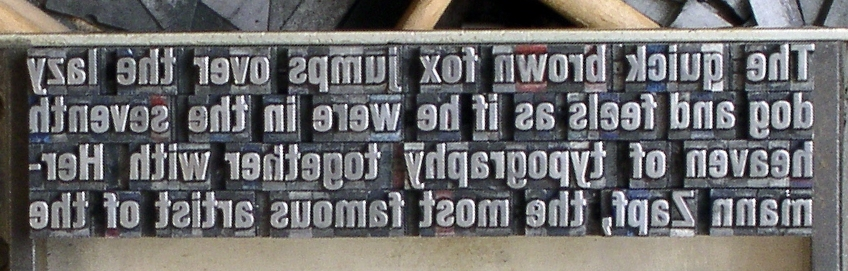
\includegraphics[width=.45\textwidth]{活版印刷字型.jpg}
	\caption{\content{由活字字型排成的英文活版}{由活字字型排成的英文活版}}
	\label{figure:由活字字型排成的英文活版}
\end{wrapfigure}
\content{電腦字型的前身是印刷字型。在沒有熒幕的時代,人們使用「活字」排印文章,就像現代人使用Word等排版軟體來排列電腦漢字那樣。「font」這個詞,最早便是指活版印刷時的一整套活字(\cref*{figure:由活字字型排成的英文活版})。活版字型的大小、線條的粗細和每個字的風格都比較接近,對於中文這種方塊字來說尤其如此。}{电脑字型的前身是印刷字型。在没有屏幕的时代,人们使用“活字”排印文章,就像现代人使用Word等排版软件来排列电脑汉字那样。“font”这个词,最早便是指活版印刷时的一整套活字(\cref*{figure:由活字字型排成的英文活版})。活版字型的大小、线条的精细和每个字的风格都比较接近,对于中文这种方块字来说尤其如此。}\par
\content{而在活字印刷術興起之前,並不存在「字型」這種概念,只有「字體(typeface)」。字體是一個很寬泛的概念,比如書法中的「楷書」,既有不足一公分的小楷,又有十幾甚至幾十公分的大楷。可以說,只要符合一定的風格,無論大小,無論粗細,都屬於同一「字體」,但它們未必是同一「字型」。舉個例子:「思源宋體」是一套字體,而「思源宋體(繁體字)Semibold 10pt」是一個具體的字型,它詳細指明了字形標準、筆畫粗細和字形大小。}{而在活字印刷术兴起之前,并不存在“字型”这种概念,只有“字体(typeface)”。字体是一个很宽泛的概念,比如书法中的“楷书”,既有不足一公分的小楷,又有十几甚至几十公分的大楷。可以说,只要符合一定的风格,无论大小,无论精细,都属于一同“字体”,但它们未必是同一“字型”。举个例子:“思源宋体”是一套字体,而“思源宋体(简体字) Semibold 10pt”是一个具体的字型,它详细指明了字型标准、笔画细粗和字型大小。}\par
\begin{figure}[H]
	\centering
	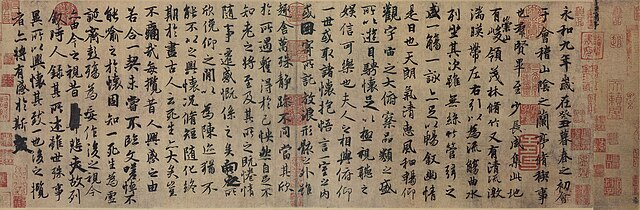
\includegraphics[height=5cm]{蘭亭集序.jpg}
	\caption{\content{〈蘭亭集序〉}{《兰亭集序》}}
	\label{figure:《蘭亭集序》}
\end{figure}
\content{在書法及早期雕版印刷中,人們只是傾向於使用相同的「字體」;至於字的大小,沒有嚴格的要求。我們看行書書法〈蘭亭集序〉(\cref*{figure:《蘭亭集序》})的排版,有的字寬,有的字窄,有的字長,有的字短,大小不一。現代圖書排版幾乎不會使用這種方式了,而是如同本書一樣,用一套字面大小相同的字型,整齊地排列文字內容。那麼它們之間有什麼區別呢?書法中的字體,又能否直接用在本書這樣的著作中呢?接下來我們會慢慢探討這些問題。}{在书法及早期雕版印刷中,人们只是倾向于使用相同的“字体”;至于字的大小,没有严格的要求。我们看行书书法《兰亭集序》(\cref*{figure:《蘭亭集序》})的排版,有的字宽,有的字窄,有的字长,有的字短,大小不一。现代图书排版几乎不会使用这种方式了,而是如同本书一样,用一套字面大小相同的字型,整齐地排列文字内容。那么它们之间有什么区别呢?书法中的字体,又能否直接用在本书这样的著作中呢?接下来我们会慢慢探讨这些问题。}\par
\subsubsection{\content{字體的兩個屬性}{字体的两个属性}}
\content{無論手寫還是印刷,文字的存在都必須依賴於特定的圖形——字形(glyph)。一款字體可以看作是在一個字集內,由風格一致的字形構成的「家族」。}{无论手写还是印刷,文字的存在都必须依赖于特定的图形——字形(glyph)。一款字体可以看作是在一个字体内,由风格一致的字形构成的“家族”。}\par
\begin{figure}[H]
	\centering
	\begin{subcaptionblock}{.3\textwidth}
		\centering
		\begin{tikzpicture}
			\node at(0,0){\fontsize{60pt}{0}\HanWangKanTan 祭};
			\node at(.12,-.05)[circle,draw,minimum size=68,line width=6]{};
		\end{tikzpicture}
		\caption{\content{勘亭流字體}{勘亭流字体}}
	\end{subcaptionblock}%
	\begin{subcaptionblock}{.3\textwidth}
		\centering
		\begin{tikzpicture}
			\node at(0,0){\fontsize{60pt}{0}\textit{祭}};
			\node at(-.05,-.05)[circle,draw,minimum size=68,line width=6]{};
		\end{tikzpicture}
		\caption{\content{標楷體}{楷體~\_GB2312}}
	\end{subcaptionblock}%
	\caption{\content{不同字體的「祭」字傳達出不同的意義}{不同字体的“祭”字传达出不同的意义}}
	\label{figure:不同字體的「祭」字傳達出不同的意義}
\end{figure}
\content{不同的字體會給人傳達出不同的印象,甚至左右人們對其含義的判斷。\cref*{figure:不同字體的「祭」字傳達出不同的意義}中的兩個「祭」字,一個是源於日本江戶時代歌舞伎文化的勘亭流字體,其舞動的外形讓人想到熱鬧、歡愉的場合,比如日式祭典;而另一個則是端正的標楷體,讓人想到肅穆、莊重的場合,比如死者的祭奠。一個喜慶,一個悲喪,它們的區別僅僅在於「換了一個字體」而已!}{不同的字体会给人传达出不同的印象,甚至左右人们对其含义的判断。\cref*{figure:不同字體的「祭」字傳達出不同的意義}中的两个“祭”字,一个是源于日本江户时代歌舞伎文化的勘亭流字体,其舞动的外形让人想到热闹、欢偷的场合,比如日式祭典;而另一个则是端正的楷体,让人想到肃穆、庄重的场合,比如死者的祭奠。一个喜庆,一个悲丧,它们的区别仅仅在于“换了一个字体”而已!}\par
\content{筆者認為,字體有兩個屬性:\textbf{工具性}和\textbf{藝術性}。工具性是指,一款字體應當準確地傳達文字的含義,使人易於閱讀和理解,盡可能避免誤讀和歧義。有些人寫的字(姑且認為每個人的手寫體都是一種字體)把「白」字寫得如同「百」字、「千」字寫得如同「干」字,導致別人閱讀起來不光很吃力,還容易認錯,這就是一種工具性比較差的字體。上文提到的勘亭流與標楷體是兩種工具性指向完全不同的字體。如果不慎用錯了,就免不了會讓人感到困惑。}{笔者认为,字体有两个属性:\textbf{工具性}和\textbf{艺术性}。工具性是指,一款字体应当准确地传达文字的含义,使人易于阅读和理解,尽可能避免误读和歧义。有些人写的字(姑且认为每个人的手写体者是一种字体)把“白”字写得如同“百”字、“千”字写得如同“干”字,导致别人阅读起来不光很吃力,还容易认错,这就是一种工具性比较差的字体。上文提到的勘亭流与楷体是两个工具性指向完全不同的字体。如果不慎用错了,就免不了会让人感到困惑。}\par
\content{而藝術性是指字體本身所展現的美感,乃至對字體創作者情操、性格的表達。同為楷書,歐陽詢的歐體剛硬險峻,顏真卿的顏體豐腴雄渾,柳公權的柳體疏朗開闊,趙孟頫的趙體圓潤清秀,不同人的字體有不同的藝術效果;當然,我們在實際生活中也可能發現有些人寫字很醜,要麼字形歪斜,要麼比例失衡,要麼字間距過大或過小,這些「醜字」的藝術性當然是比不上歐、顏、柳、趙的。}{而艺术性是指字体本身所展现的美感,乃至对字体创作者情操、性格的表达。同为楷书,欧阳询的欧体刚硬险峻,颜真卿的颜体丰腴雄浑,柳公权的柳体疏朗开阔,赵孟頫的赵体圆润清秀,不同人的字体有不同的艺术效果;当然,我们在实际生活中也可能发现有些人写字很丑,要么字形歪斜,要么比例失衡,要么字间距过大或过小,这些“丑字”的艺术性当然是比不上欧、颜、柳、赵的。}\par
\content{工具性與藝術性只是評價字體的兩個維度,它們之間未必是對立關係。歐、顏、柳、趙的書法既有十足的美感,又不妨礙人們對內容的閱讀理解,可以說在藝術性和工具性上都相當優秀。但有些人寫的「醜字」既不好看,又讓別人根本看不懂,可以說在藝術性和工具性方面都相當失敗。}{工具性与艺术性只是评价字体的两个维度,它们之间未必是对立关系。欧、颜、柳、赵的书法既既有十足的美感,又不妨碍人们对内容的阅读理解,可以说在艺术性和工具性上都相当优秀。但有些人写的“丑字”既不好看,又让别人根本看不懂,可以说在艺述性和工具性方面者相当失败。}\par
\begin{wrapfigure}{O}{.4\textwidth}
	\centering
	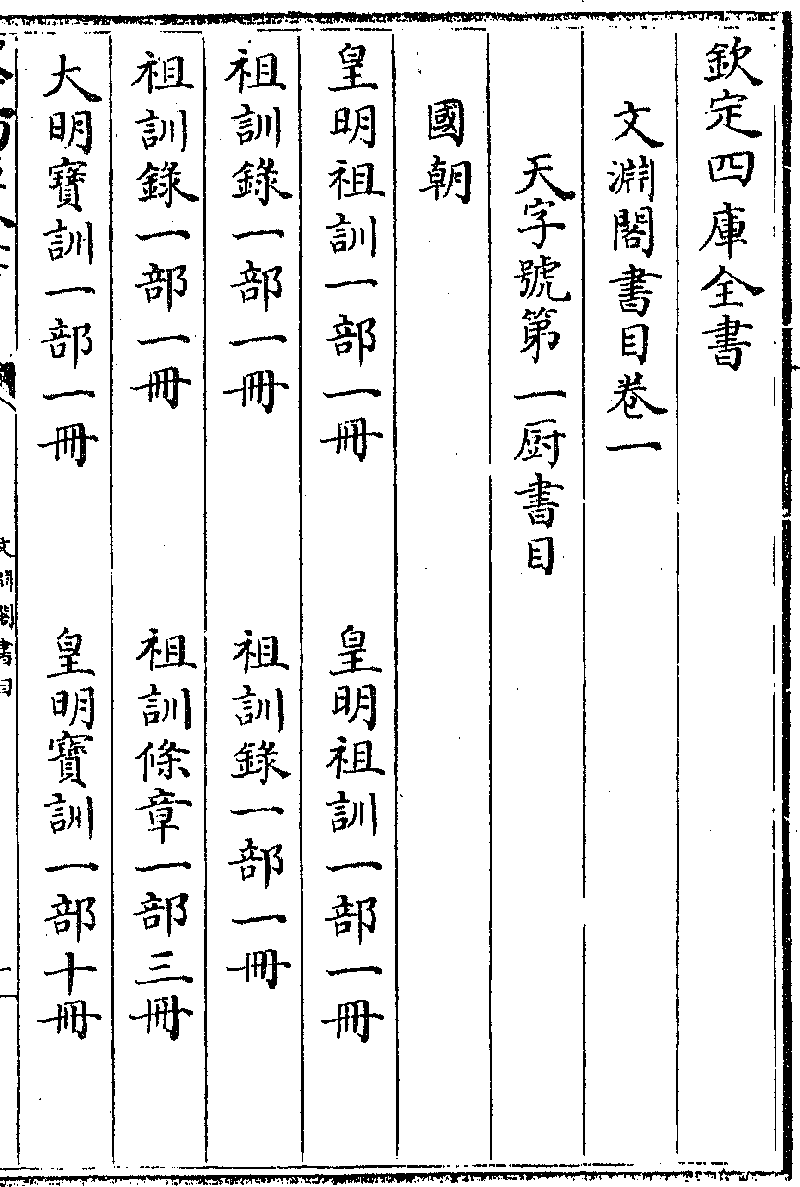
\includegraphics[width=.4\textwidth]{文淵閣四庫全書-書影.png}
	\caption{\content{四庫全書中的館閣體}{四库全书中的馆阁体}}
	\label{figure:四庫全書中的館閣體}
\end{wrapfigure}
\content{草書的工具性比較低,因為只有經過草書訓練的人才能看懂;旁人讀起來就會很吃力。至於狂草,那更是純粹的藝術品了。因此,古人在需要工具性字體的場合,比如科舉、書信、記事,一般不會使用草書,而是使用楷書,或者介於楷、草之間的行書——楷書雖好,但寫起來太慢了。}{草书的工具性比较低,因为只有经过草书训练的人才能看懂;旁人读起来就会很吃力。至于狂草,那更是纯粹的艺术品了。因此,古人在需要工具性字体的场合,比如科举、书信、记事,一般不会使用草书,而是使用楷书,或者介于楷、草之间的行书——楷书虽好,但写起来太慢了。}\par
\content{楷書中的分支「館閣體」是清朝公文的標準字體。無論讀書人考科舉,還是大臣上書,都必須要使用館閣體來行文(\cref*{figure:四庫全書中的館閣體})。館閣體強調書寫字形、大小、粗細統一,要求每一個字都方正整齊、墨色烏亮,像是規定了一套異常嚴格的字體標準,要求人們照做。也正因如此,每個人寫出來的字看上去都差不多。}{楷书中的分支“馆阁体”是清朝公文的标准字体。无论读书人考科举,还是大臣上书,都必须要使用馆阁体来行文(\cref*{figure:四庫全書中的館閣體})。馆阁体强调书写字形、大小、粗细统一,要求每一个字都方正整齐、墨色乌亮,像是规定了一套异常严格的字体标准,要求人们照做。也正因如此,每个人写出来的字看上去都差不多。}\par
\content{這種「千手雷同」的字體缺少個性,且太拘謹,不自然,所以很多書法愛好者對此並不欣賞。周星蓮說這字體是「土龍木偶,毫無意趣」\footnote{語出〈臨池管見〉。其實周星蓮指責的是「台閣體」,而台閣體又是館閣體的前身,二者之間共性頗多。所以可以說,他也是在批評後來的館閣體。},也有一定的道理。館閣體的工具色彩太重,於是其藝術色彩便打了折扣,這與草書的情況是恰巧相反的。}{这种“千手雷同”的字体缺少个性,且太拘谨,不自然,所以很多书法爱好者对此并不欣赏。周星莲说这字体是“土龙木偶,毫无意趣”\footnote{语出《临池管见》。其实周星莲指责的是“台阁体”,而台阁体又是馆阁体的前身,二者之间共性颇多。所以可以说,他也是在批评后来的馆阁体。},也有一定的道理。馆阁体的工具色彩太重,于是其艺术色彩便打了折扣,这与草书的情况是恰巧相反的。}\par
\begin{figure*}[p]\centering
	\begin{subcaptionblock}{.32\textwidth}\centering
		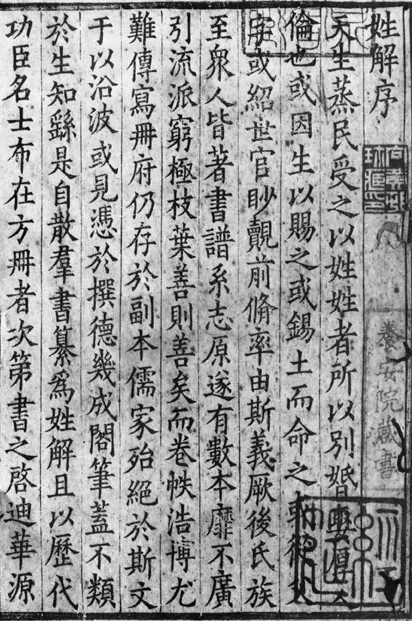
\includegraphics[trim={88pt 65pt 36pt 60pt},clip,height=9cm]{浙江刊本-姓解.jpeg}
		\caption{\content{\parbox[c]{4em}{\centering 浙江刊本\\《姓解》}}{\parbox[c]{4em}{浙江刊本\\《姓解》}}}
	\end{subcaptionblock}
	\begin{subcaptionblock}{.32\textwidth}\centering
		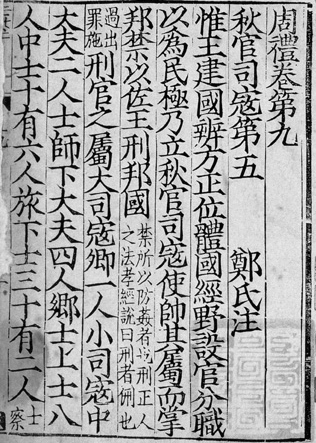
\includegraphics[trim={35pt 20pt 38pt 10pt},clip,height=9cm]{四川刊本-周禮.jpeg}
		\caption{\content{\parbox[c]{4em}{\centering 四川刊本\\《周禮》}}{\parbox[c]{4em}{\centering 四川刊本\\《周礼》}}}
	\end{subcaptionblock}
	\begin{subcaptionblock}{.32\textwidth}\centering
		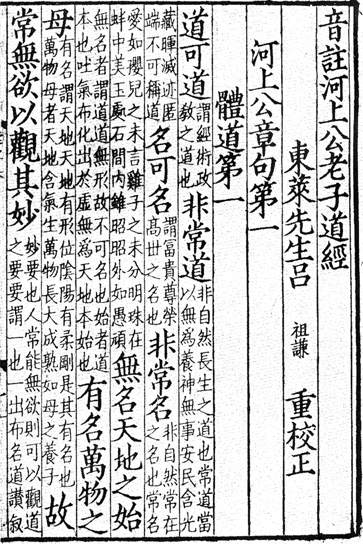
\includegraphics[trim={82pt 60pt 10pt 20pt},clip,height=9cm]{福建刊本-音注河上公老子道經.jpg}
		\caption{\content{\parbox[c]{10em}{\centering 福建刊本\\《音注河上公老子道經》}}{\parbox[c]{10em}{\centering 福建刊本\\《音注河上公老子道经》}}}
	\end{subcaptionblock}
	\caption{\content{宋朝刊本書影}{宋朝刊本书影}}
	\label{figure:宋朝刊本書影}
\end{figure*}
\begin{figure*}[p]\centering
	\begin{subcaptionblock}{.32\textwidth}\centering
		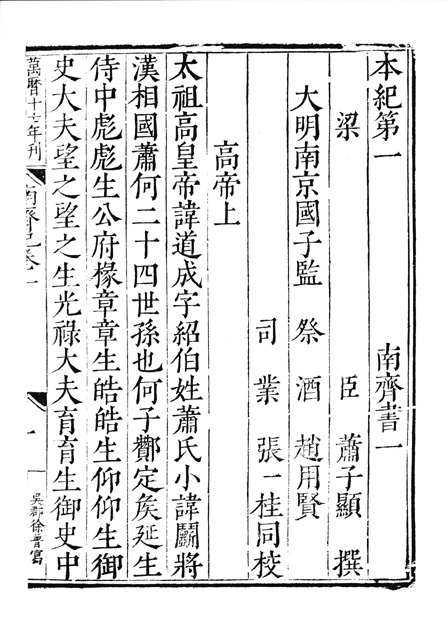
\includegraphics[trim={91pt 85pt 110pt 58pt},clip,height=9cm]{南京國子監刊本-南齊書.jpeg}
		\caption{\content{\parbox[c]{7em}{\centering 南京國子監刊本《南齊書》}}{\parbox[c]{7em}{\centering 南京国子监刊本《南齐书》}}}
	\end{subcaptionblock}
	\begin{subcaptionblock}{.32\textwidth}\centering
		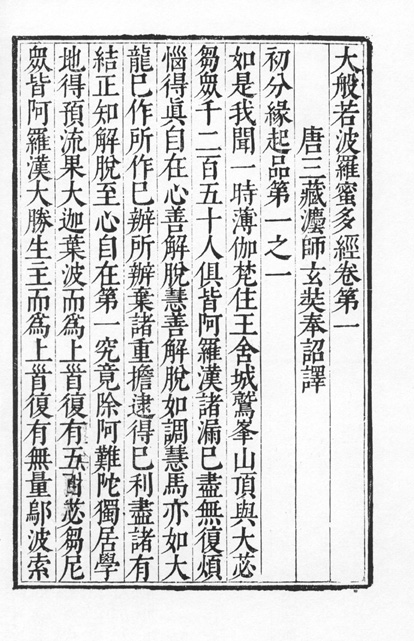
\includegraphics[trim={95pt 125pt 81pt 70pt},clip,height=9cm]{楞嚴寺刊本-嘉興藏.jpeg}
		\caption{\content{\parbox[c]{5em}{\centering 楞嚴寺刊本\\《嘉興藏》}}{\parbox[m]{5em}{楞严寺刊本《嘉兴藏》}}}
	\end{subcaptionblock}
	\begin{subcaptionblock}{.32\textwidth}\centering
		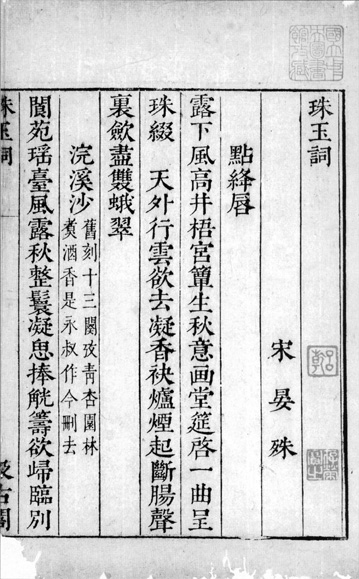
\includegraphics[trim={61pt 72pt 63pt 93pt},clip,height=9cm]{毛晉汲古閣刊本-宋名家詞.jpeg}
		\caption{\content{\parbox[c]{7em}{\centering 毛晉汲古閣刊本\\《宋名家詞》}}{\parbox[c]{7em}{\centering 毛晋汲古阁刊本\\《宋名家词》}}}
	\end{subcaptionblock}
	\caption{\content{明朝刊本書影}{明朝刊本书影}}
	\label{figure:明朝刊本書影}
\end{figure*}
\subsubsection{\content{從書法到印刷}{从书法到印刷}}
\content{印刷術出現在隋唐時期,但真正繁榮是在宋朝以後。宋朝三大印刷集中地——浙江、四川、福建——的刊本字體,就分別繼承了唐朝歐陽詢、顏真卿、柳公權的書法風格(\cref*{figure:宋朝刊本書影})。這一時期的印刷字體尚與書法相似;但畢竟刻刀不如毛筆那樣富有變化,所以印刷字體很難做到書法級別的藝術性。}{印刷术出现在隋唐时期,但真正繁荣是在宋朝以后。宋朝三大印刷集中地——浙江、四川、福建——的刊本字体,就分别继承了唐朝欧阳询、颜真卿、柳公权的书法风格(\cref*{figure:宋朝刊本書影})。这一时期的印刷字体尚与书法相似;但毕竟刻刀不如笔笔那样富有变化,所以印刷字体很难做到书法级别的艺术性。}\par
\content{到了明朝以後,印刷字體中的書法氣息逐漸淡化,並演變出了一種「橫細竪粗撇如刀,點如瓜子捺如掃」的新字體——明體(\cref*{figure:明朝刊本書影})。明體字的橫畫基本是水平的(宋刊本中的橫畫則是明顯偏斜的),橫畫的末端有小三角形的襯線\footnote{襯線是一種裝飾線。}(宋刻本中的橫畫也帶有襯線,但不如明體那樣有很高的一致性),並且橫畫細、竪畫粗(宋刻本中的橫竪筆畫粗細相似)。}{到了明朝以后,印刷字体中的书法气息逐渐淡化,并演变出了一种“横细竖粗撇如刀,点如瓜子捺如扫”的新字体——明体(\cref*{figure:明朝刊本書影})。明体字筆畫方正,它的横画基本是水平的(宋刊本中的横画则是明显偏斜的),横画的末端有小三角形的衬线\footnote{衬线是一种装饰线。}(宋刊本中的横画也带有衬线,但不如明体那样有很高的一致性),并且横画细、竖画粗(宋刻本中的横竖笔画粗细相似)。}\par
\content{變化的不只是字體。相比於宋刊本,明刊本的排版也十分整齊,如同是在方格紙上寫出來的一樣。其實,在閱讀大篇幅文本時,這種整齊的排版更便於閱讀,而像宋刻本那樣大小不一的字體就會更容易引起視疲勞。}{变化的不只是字体。相比于宋刊本,明刊本的排版也十分整齐,如同是在方格纸上写出来的一样。其实,在阅读大篇幅文本时,这种整齐的排版更便于阅戾,而像宋刻本那样大小不一的字体就会更容易引起视疲劳。}\par
\content{但是文人們對此可不買賬。明清時期有許多文人嚴厲地批評這種字體,覺得它把漢字本來的美感都破壞了:}{但是文人们对此可不买账。明清时期有许多文人严厉地批评这种字体,觉得它把汉字本来的美感者破坏了:}
\begin{boxquote}{\content{錢泳《履園叢話·藝能》}{钱泳《履园丛话·艺能》}}
	\content{刻書以宋刻為上,至元時翻宋,尚有佳者。有明中葉寫書匠改為方筆,非顏非歐,已不成字,近時則愈惡劣,無筆畫可尋矣。}{刻书以宋刻为上,至元时翻宋,尚有佳者。有明中叶写书匠改为方笔,非颜非欧,已不成字,近时则愈恶劣,无笔画可寻矣。}
\end{boxquote}
\content{文人們對明體的批評與對館閣體的批評很相像;而這些批評的問題就在於——文人們是在用審視藝術的眼光審視工具性字體。實際上,這種由書法字體到印刷字體(如明體)的轉變既不是墮落,也不是升華,只是因為讀寫媒介與需求改變了,字體「工具」自然也就跟著改變了,僅此而已。而從工具性的角度上講,明體正是「整齊、清晰、易辨」的典範。}{文人们对明体的批评与对馆阁体的批评很相像;而这些批评的问题就在于——文人们是在用审视艺术的眼光审视工具性字体。实际上,这种由书法字体到印刷字体(如明体)的转变既不是堕落,也不是升华,只是因为读写媒介与需求改变了,字体“工具”自然也就跟着改变了,仅此而已。而从工具性的角度上讲,明体睚是“整齐、清晰、易辨”的典范。}\par
\begin{figure}[H]\centering
	\begin{subcaptionblock}{.2\textwidth}\centering
		
\includegraphics[height=2cm]{楷書/永-沈尹默.png}
		\caption*{\content{楷書}{楷书}}
		\label{figure:楷書-永}
	\end{subcaptionblock}%
	\begin{subcaptionblock}{.2\textwidth}\centering
		\begin{tikzpicture}
			\node at(0,0){\fontsize{60pt}{0}永};
		\end{tikzpicture}
		\caption*{\content{明體}{明体}}
	\end{subcaptionblock}%
	\begin{subcaptionblock}{.2\textwidth}\centering
		\begin{tikzpicture}
			\node at(0,0){\fontsize{60pt}{0}\content{\twsans 永}{\zhsans 永}};
		\end{tikzpicture}
		\caption*{\content{黑體}{黑体}}
	\end{subcaptionblock}%
	\caption{\content{書法楷書、明體與黑體的「永」字}{书法楷书、明体与黑体的“永”字}}
\end{figure}
\content{況且,從現代人的視角來看,明體已經相當有書法氣息。它的小三角形襯線是在模仿楷書的收筆;捺由細變粗、撇由粗變細也對應毛筆運筆過程中加壓或放鬆的動作,比沒有襯線的黑體來說,顯得傳統很多。也正因如此,明體廣泛用於正文的排版、印刷之中,是一類能夠傳達權威感、專業感、正式感的字體。本書的正文幾乎都是使用思源宋體來排版的,它就是明體的一種。}{况且,从现代人的视角来看,明体已经相当有书法气息。它的小三角形衬线是在模仿楷书的收笔;捺由细变粗、撇由粗变细也对应毛笔运笔过程中加压或放松的动作,比没有衬线的黑体来说,显得传统很多。也正因如此,明体广泛用于正文的排版、印刷之中,是一类能够传达权威感、专业感、正式感的字体。本书的正文几乎者是使用思源宋体来排版的,它就是明体的一种。}\par
\content{讀者看到這裡或許會有些迷惑——為什麼思源宋體是一種明體?下面我們就來談談這個名稱背後的故事。}{读者看到这里或许会有些迷惑——为什么思源宋体是一种明体?下面我们就来谈谈这个名称背后的故事。}\par
\subsubsection{\content{「宋體」非宋}{“宋体”非宋}}
\content{前文已經說過,宋刻本字體與明刻本有著顯著的不同。如果我們還要再細分的話,其實宋、元、明、清歷朝歷代的字體都是有區別的\footnote{讀者可以透過\href{https://www.kinkido.net/STUDY/study.html}{活字書体の基礎講座|欣喜堂}了解到關於不同時期字體的詳細知識。}。但如今,我們卻把各有特色的字體統統劃作「明體」一類——這也就算了,可是有不少人卻又叫它「宋體」,簡直亂成一團。}{前文已经说过,宋刻本字体与明刻本有着显著的不同。如果我们还要再细分的话,其实宋、元、明、清历朝历代的字体者是有区别的\footnote{读者可以透过\href{https://www.kinkido.net/STUDY/study.html}{活字書体の基礎講座|欣喜堂}了解到关于不同时期字体的详细知识。}。但如今,我们却把各有特色的字体统统划作“明体”一类——这也就算了,可是有不少人却又叫它“宋体”,简直乱成一团。}\par
\content{其實這種字體起初就是明朝的字體,也正是叫做明體,只是後來有人把這種字體稱作「宋體」\footnote{坊間流傳的一種說法是,康熙皇帝曾在刻印《文獻通考》修訂版時指示「此後刻書,凡方體稱宋體字,楷書均稱軟字」。可是,筆者完全沒有找到這段話的出處,因此這個說法究竟是真是假,還很難確定。},於是以訛傳訛,最後大家都叫它「宋體」了。但日本人沒有受到這種訛傳的影響,他們考據發現這種字體起源於明朝,於是叫它「明體」。這個名稱又隨著技術引進,傳播到台港澳地區\footnote{後來台灣教育部也開始使用「宋體」這個名字。不過在台灣民間,「明體」這個名字依然深入人心。};而大陸則一直使用清初沿襲下來的「宋體」之名。正因如此,同一套字體便有了兩個名字。}{其实这种字体起初就是明朝的字体,也正是叫做明体,只是后来有人把这种字体称作“宋体”\footnote{坊间流传的一种说法是,康熙皇帝曾在刻印《文献通考》修订版时指示“此后刻书,凡方体称宋体字,楷书均称软字”。可是,笔者完全没有找到这段话的出处,因此这个说法究竟是真是假,还很难确定。},于是以讹传讹,最后大家都叫它“宋体”了。但日本人没有受到这种讹传的影响,他们考据发现这种字体起源于明朝,于是叫它“明体”。这个名称又随著技术引进,传播到台港澳地区\footnote{后来台湾教育部也开始使用“宋体”这个名字。不过在汉湾民间,“明体”这个名字依然深入人心。};而大陆则一直使用清初沿袭下来的“宋体”之名。正因如此,同一套字体便有了两个名字。}\par
\content{可是文人們終究還是喜歡宋版書那樣的字體。1915年,丁善之、丁輔之兄弟二人就仿照宋朝刻本中的字體,制作了新的字體。可是「宋體」這個名字已經被明體張冠李戴用去了,於是只好給它起名為「仿宋體」,以作區分。}{可是文人们终究还是喜欢宋版书那样的字体。1915年,丁善之、丁辅之兄弟二人就仿照宋朝刻本中的字体,制作了新的字体。可是“宋体”这个名字已经被明体张冠李戴用去了,于是只好给它起名为“仿宋体”,以作区分。}\par
\begin{figure}[b]\centering
	\vspace{-2.3ex}
	\footnoterule
	\begin{minipage}{.9\textwidth}
		\content{\fontshow{全字庫正宋體(明體/宋體)}{\TWSung}}{\fontshow{方正书宋(宋体)}{\FZShuSongZ01S}}
		\content{\fontshow{王漢宗中仿宋繁(仿宋)}{\HanWangFangSongMedium}}{\fontshow{方正仿宋简体(仿宋)}{\FZFangSongZ02S}}
	\end{minipage}
\end{figure}
\content{仿宋體具有很鮮明的宋刻本字體特色——偏斜的橫畫,粗細一致的橫竪筆,以及更接近手寫字的質感,因而備受人們的喜愛。據說,因為許多文人都想要用仿宋體來印刷自己的名片,以致中華書局成立了專門的「名片部」,在各省分店接單印製名片,可見文人對仿宋體的喜愛。}{仿宋体具有很鲜明的宋刻本字体特色——偏斜的横画,粗细一致的横竖笔,以及更接近手写字的质感,因而备受人们的嘉爱。据说,因为许我文人都想要用仿宋体来印刷自己的名版,以致中华书局成立了专门的“名片部”,在各省分店接单印制名片,可见文人对仿宋体的喜爱。}\par
\content{總而言之,現今兩岸四地所稱的「明體」和「宋體」其實是一回事,都是模仿明刻本風格的字體;而「仿宋體」其實才是真正模仿宋刻本設計出來的字體。}{总而言之,现今两岸四地所称的“明体”和“宋体”其实是一回事,都是模仿明刻本风格的字体;而“仿宋体”其实才是真正模仿宋刻本设计出来的字体。}\par
\subsubsection{\content{黑體、圓體}{黑体、圆体}}
\content{說到黑體,可能我們最先想到它的「黑」。之所以會產生這種印象,是因為人們通常會在白底黑字旳場景下閱讀文字,而黑體較粗的線條使得整個視覺空間被更多黑色的部分所佔據,所以我們會覺得它很「黑」。}{说到黑体,可能我们最先想到它的“黑”。之所以会产生这种印象,是因为人们通常在白底黑字的场景下阅读文字,而黑体较粗的线条使得整个视觉空间被更多黑色的部分所占据,所以我们会觉得它很“黑”。}\par
\content{然而,不是任何一種看上去很「黑」的字型都可以叫做「黑體」;也不是任何一款「黑體」都一定要很「黑」!我們在Word排版中可能經常需要對明體「加粗」來表示強調,其實這根本不能算一種黑體,只能說是較粗的明體而已。另外,有些線條很細的字型雖然看上去並沒有給人很「黑」的印象,但卻是實打實的黑體。因此,僅憑線條的粗細和整字的觀感來判定一個字是不是黑體,這是很容易出錯的。}{然而,不是任何一种看上去很“黑”的字型者可以叫做“黑体”;也不是任何一款“黑体”都一定要很“黑”!我们在Word排版中可能经常需要对宋体“加粗”来表示强调,其实这根本不能算一种黑体,只能说是较粗的宋体而已。另外,有些线条很细的字型虽然看上去并没有给人很“黑”的印象,但却是实打实的黑体。因此,仅凭线条的粗细和整字的观感来判定一个字是不是黑体,这是很容易出错的。}\par
\content{黑體有一些比較典型的特徵,比如橫平竪直(與仿宋體不同),筆畫粗細比較一致(與明體有不少差異),襯線較淡甚至完全沒有。}{黑体有一些比较典型的特征,比如横平竖直(与仿宋体不同),笔画粗细比较一致(与宋体有不少差异),衬线较淡甚至完全没有。}
\begin{figure}[H]\centering
	\begin{subcaptionblock}{.25\textwidth}\centering
		{\GenRyuMinTWTTF\fontsize{40pt}{0}永}
		\caption*{\content{源流明體}{源流明体(宋体)}}
	\end{subcaptionblock}%
	\begin{subcaptionblock}{.25\textwidth}\centering
		{\FZHeiB01S\fontsize{40pt}{0}永}
		\caption*{\content{方正黑體簡體}{方正黑体简体}}
	\end{subcaptionblock}%
	\begin{subcaptionblock}{.25\textwidth}\centering
		{\NotoSansCJKTCMedium\fontsize{40pt}{0}永}
		\caption*{\content{思源黑體 Medium}{思源黑体 Medium}}
	\end{subcaptionblock}%
	\begin{subcaptionblock}{.25\textwidth}\centering
		{\HanWangHeiHeavy\fontsize{40pt}{0}永}
		\caption*{\content{王漢宗特黑體繁}{王汉宗特黑体繁}}
	\end{subcaptionblock}%
	\caption{\content{源流明體與其它三款黑體}{源流明体与其它三款黑体}}
	\label{figure:源流明體與其它三款黑體}
\end{figure}
\content{\cref*{figure:源流明體與其它三款黑體}中所列舉的三種黑體各有特色。讀者若是仔細觀察,一定能發現,方正黑體的筆畫末端略微加粗,呈現出「喇叭頭」的形狀,且撇捺處有明顯的線條粗細變化;思源黑體則沒有喇叭頭,每一筆都一樣粗\footnote{讀者如果仔細測量,會發現思源黑體的橫畫比竪畫略細一些,並不存在「測量」意義上的一致。這是因為,人眼會產生視錯覺,把相同粗細的橫線看得比竪線更粗;於是字體設計者就需要把橫線畫得比竪線略細,從而達到「視覺」意義上的一致。更多詳細資訊可參考\href{http://designwithfontforge.com/en-US/Trusting_Your_Eyes.html}{Design With FontForge: Trusting Your Eyes}。};王漢宗特黑體更是把畫筆的末端切成圓角,已經有了接近於圓體的風格。}{\cref*{figure:源流明體與其它三款黑體}中所列举的三种黑体各有特色。读者若是仔细观察,一定能发现,方正黑体的笔画末端略微加粗,呈现出“喇叭头”的形状,且撇捺处有明显的线条粗细变化;思源黑体则没有喇叭头,每一笔者一样粗\footnote{读者如果仔细测量,会发现思源黑体的横画比竖画略细一些,并不存在“测量”意义上的一致。这是因为,人眼会产生视错觉,把相同粗细的横线看得比竖线更粗;于是字体设计者就需要把横线画得比竖线略细,从而达到“视觉”意义上的一致。更多详细信息可参考\href{http://designwithfontforge.com/en-US/Trusting_Your_Eyes.html}{Design With FontForge: Trusting Your Eyes}。};王汉宗特黑体更是把笔画的末端切成圆角,已经有了接近于圆体的风格。}\par
\begin{figure}[H]\centering
	\begin{subcaptionblock}{.25\textwidth}\centering
		\begin{tikzpicture}
			\clip(-2.5,.14)circle(.8);
			\node[inner sep=0pt]at(0,0){\FZHeiB01S\fontsize{200pt}{0}永};
		\end{tikzpicture}
		\caption*{\content{方正黑體簡體}{方正黑体简体}}
	\end{subcaptionblock}%
	\begin{subcaptionblock}{.25\textwidth}\centering
		\begin{tikzpicture}
			\clip(-2.5,.145)circle(.8);
			\node[inner sep=0pt]at(0,0){\NotoSansCJKTCMedium\fontsize{200pt}{0}永};
		\end{tikzpicture}
		\caption*{\content{思源黑體 Medium}{思源黑体 Medium}}
	\end{subcaptionblock}%
	\begin{subcaptionblock}{.25\textwidth}\centering
		\begin{tikzpicture}
			\clip(-2.5,.244)circle(.8);
			\node[inner sep=0pt]at(0,0){\HanWangHeiHeavy\fontsize{200pt}{0}永};
		\end{tikzpicture}
		\caption*{\content{王漢宗特黑體繁}{王汉宗特黑体繁}}
	\end{subcaptionblock}%
	\caption{\content{三款黑體的筆畫細節}{三款黑体的笔画细节}}
	\label{figure:三款黑體的筆畫細節}
\end{figure}
\begin{figure}[b]\centering
	\vspace{-2.3ex}
	\footnoterule
	\begin{minipage}{.9\textwidth}
 		\fontshow{\content{有愛圓體}{有爱圆体}}{\content{\NowarRoundedTW}{\NowarRoundedCN}}
	\end{minipage}
\end{figure}
\content{熟悉歐文的人可能會想到歐文中的無襯線體(sans-serif),並把它與中日韓文字中的黑體等同起來。其實,黑體也是可以有襯線的!方正黑體、小塚黑體等很多類型的黑體都有類似於襯線的設計。所以歐文中的「無襯線體」很難對應到中日韓文字中的具體一類。不過,多數情況下黑體能與歐文中的無襯線體較好地搭配起來,因此將他們並舉也是沒問題的。}{熟悉欧文的人可能会想到欧文中的无衬线体(Sans-serif),并把它与中日韩文字中的黑体等同起来。其实,黑体也是可以有衬线的!方正黑体、小塚黑体等很多类型的黑体都有类似于衬线的设计。所以欧文中的“无衬线体”很难对应到中日韩文字中的具体一类。不过,多数情况下黑体能与欧文中的无衬线体罗好地搭配丐来,因此将他们并举也不没问题的。}\par
\content{圓體與黑體有很多相似之處,比如橫平竪直,線條粗細基本一致等等。最明顯的區別在於,圓體的筆畫末端是圓角的。有些圓體的結構比較鬆散,再加上有圓角造型,也容易給人以可愛的印象。}{圆体与黑体有很多相似之处,比如横平竖直,线条粗细基本一致等等。最明显的区别在于,圆体的笔画末端是圆角的。有些圆体的结构比较松散,再加上有圆角造型,也容易给人以可爱的印象。}\par
\subsubsection{\content{字重與偽粗體}{字重与伪粗体}}
\content{無論哪一種字體,都可以有線條粗細的區分——有很粗的明體,也有很細的黑體。衡量一個字型線條粗細的指標叫做\textbf{字重(weight)}。有些字體設計者會設計出不同字重的一系列字型,並把它們打包成一個\textbf{字型家族(font family)}。比如說,思源系列的字體就設計了七種字重,讓使用者可以自由選擇不同粗細的字型。}{无论哪一种字体,都可以有线条粗细的区分——有很粗的宋体,也有很细的黑体。衡量一个字型线条粗细的指标叫做\textbf{字重(weight)}。有些字体设计者会设计出不同字重的一系列字型,并把它们打包成一个\textbf{字型家族(font family)}。比如说,思源系列的字体就设计了七种字重,让使用者可以自由选择不同粗细的字型。}\par
\begin{figure}[H]\centering
	\begin{subcaptionblock}{.142\textwidth}\centering
		{\NotoSerifCJKTCExtraLight\fontsize{40pt}{0}永}
		\caption*{ExtraLight}
	\end{subcaptionblock}%
	\begin{subcaptionblock}{.142\textwidth}\centering
		{\NotoSerifCJKTCLight\fontsize{40pt}{0}永}
		\caption*{Light}
	\end{subcaptionblock}%
	\begin{subcaptionblock}{.142\textwidth}\centering
		{\NotoSerifCJKTC\fontsize{40pt}{0}永}
		\caption*{Regular}
	\end{subcaptionblock}%
	\begin{subcaptionblock}{.142\textwidth}\centering
		{\NotoSerifCJKTCMedium\fontsize{40pt}{0}永}
		\caption*{Medium}
	\end{subcaptionblock}%
	\begin{subcaptionblock}{.142\textwidth}\centering
		{\NotoSerifCJKTCSemiBold\fontsize{40pt}{0}永}
		\caption*{SemiBold}
	\end{subcaptionblock}%
	\begin{subcaptionblock}{.142\textwidth}\centering
		{\NotoSerifCJKTCBold\fontsize{40pt}{0}永}
		\caption*{Bold}
	\end{subcaptionblock}%
	\begin{subcaptionblock}{.142\textwidth}\centering
		{\NotoSerifCJKTCBlack\fontsize{40pt}{0}永}
		\caption*{Black}
	\end{subcaptionblock}%
	\caption{\content{思源宋體的七種字重}{思源宋体的七种字重}}
	\label{figure:思源宋體的七種字重}
\end{figure}
\content{讀者一定能發現,這七種字重雖然看起來粗細不同,但是它們的橫畫其實都一樣細,變化的只是竪畫、撇捺和襯線的粗細。而且,字重不同,筆畫的造型也有一定的變化——請看「永」字的第一筆(點),它不是等比例地「變大」,而是只在某些特定方向上把線條加寬了。}{读者一定能发现,这七种这字重虽然看起来粗细不同,但是它们的横画其实都一样细,变化的只是竖画、撇捺和衬线的粗细。而且,字重不同,笔画的造型也有一定的变化——请看“永”字的第一笔(点),它不是等比例地“变大”,而是只在某些特定方向上把线条加宽了。}\par
\content{而在實際排版中,人們有時會使用\textbf{偽粗體(fake bold)}技術。偽粗體的處理方法就是直接等比例地加粗線條,從而達到「看上去很粗」的效果。可是,偽粗體的加粗效果如何呢?我們看一下\cref*{figure:偽粗體與真粗體的區別}就能知道答案。}{而在实际排版中,人们有时会使用\textbf{伪粗体(fake bold)}技术。伪粗体的处理方法就是直接等比例地加粗线条,从而达到“看上去很粗”的效果。可是,伪粗体的加粗效果如何呢?我们看一下\cref*{figure:偽粗體與真粗體的區別}就能知道答案。}\par
\begin{figure}[H]\centering
	\begin{subcaptionblock}{.142\textwidth}\centering
		{\NotoSerifCJKTCExtraLight\fontsize{40pt}{0}國}
		\caption*{\centering\content{思源宋體\\ExtraLight}{思源宋体\\ExtraLight}}
	\end{subcaptionblock}%
	\begin{subcaptionblock}{.142\textwidth}\centering
		{\NotoSerifCJKTCExtraLight\fontsize{40pt}{0}\fakebf[2]{國}}
		\caption*{\centering\content{ExtraLight偽粗體}{ExtraLight伪粗体}}
	\end{subcaptionblock}%
	\begin{subcaptionblock}{.142\textwidth}\centering
		{\NotoSerifCJKTCBlack\fontsize{40pt}{0}國}
		\caption*{\centering\content{思源宋體\\Black}{思源黑体\\Black}}
	\end{subcaptionblock}%
	\begin{subcaptionblock}{.142\textwidth}\centering
		{\NotoSansCJKTCMedium\fontsize{40pt}{0}國}
		\caption*{\centering\content{思源黑體\\Black}{思源黑体\\Black}}
	\end{subcaptionblock}%
	\caption{\content{偽粗體與真粗體的區別}{伪粗体与真粗体的区别}}
	\label{figure:偽粗體與真粗體的區別}
\end{figure}
\content{對比一下就不難發現,明體字經過偽粗體處理之後所有筆畫都加粗了,於是或多或少有了些黑體的特徵\footnote{或許人們常常把「黑體」和「粗體」混淆也是因為這個——Word的「加粗」其實是偽粗體!}。不過話說回來,在正文中把明體改為風格近似的黑體來表示強調,這是無可厚非的;真正的問題在於,偽粗體字形的空間分布已經嚴重失衡了。}{对比一下就不难发现,宋体字经过伪粗体处理之后所有笔画都加粗了,于是或多或少有了些黑体的特征\footnote{或许人们常常把“黑体”和“粗体”混淆也是因为这个——Word的“加粗”其实是伪粗体!}。不过话说回来,在正文中把宋体改为风格近似的黑体来表示强调,这是无可厚非的;真正的问题在于,伪粗体字型的空间分布已经严重失衡了。}\par
\content{讀者請看,在思源宋體ExtraLight字型中,內部的「或」字與外邊的「囗」旁之間存在有一定的空隙,於是整個字形看起來並不擁擠;思源宋體Black和思源黑體Black的筆畫較粗,但字型設計者把「或」字所佔的空間給收窄了(讀者測量一下便能得知),於是仍然可以保持這種空間上的平衡;然而思源宋體ExtraLight加粗得到的偽粗體字卻沒辦法調整空間了,只能任由原本分開的筆畫粘在一起——這就是空間分布上的失衡。}{读者请睦,在思源宋体ExtraLight字型中,内部的“或”字与外边的“囗”旁之间存在有一定的空隙,于是整个字型看起来并不拥挤;思源宋体Black和思源黑体Black的笔画较粗,但字型设计者把“或”字所占的空间给收窄了(读者测量一下便能得知),于是仍然可以保持这种空间上的平衡;然而思源宋体ExtraLight加粗得到的伪粗体字却没办法调整空间了,只能任由原本分开的笔画粘在一起——这就是空间分布上的失衡。}\par
\content{因此,如果一款字體擁有不同的字重,那麼我們應當盡量使用「不同的字重」來表示粗體,避免使用偽粗體。但是有些字體只有單獨一款字重,那麼我們就只能使用偽粗體了。}{因此,如果一款字体拥有不同的字重,那么我们应当尽量使用“不同的重”来表示粗体,避免使用伪粗体。但是有些字体只有单独一款字重,那么我们就只能使用伪粗体了。}\par
\subsubsection{\content{字形標準}{字形标准}}
\content{經常看不同字體的人,一定能發現,同一個字,在不同字體中有不同的寫法。這種寫法上的差異不是筆畫粗細、造型上的區別,而是字形組成部件上的區別。}{经常看不同字体的人,一定能发现,同一个字,在不同字体中有不同的写法。这种写法上的差异不是笔画粗细、造型上的区别,而是字形组成部件上的区别。}\par
\content{筆畫粗細指的是字重,上文已有介紹,這裡就不再贅述;而筆畫造型的區別是指同樣筆畫的形態差異。}{笔画粗细指的是字重,上文已有介绍,这里就不再赘述;而笔画造型的区别是指同样笔画的形态差异。}\par
\begin{figure}[H]\centering
	\begin{subcaptionblock}{.142\textwidth}\centering
		{\HanWangLiSuMedium\fontsize{47pt}{0}景}
		\caption*{\content{隸書體}{隶书体}}
	\end{subcaptionblock}%
	\begin{subcaptionblock}{.142\textwidth}\centering
		{\fontsize{43pt}{0}\textit{景}}
		\caption*{\content{楷體}{楷体}}
	\end{subcaptionblock}%
	\begin{subcaptionblock}{.142\textwidth}\centering
		{\NotoSansCJKTCBold\fontsize{40pt}{0}景}
		\caption*{\content{黑體}{黑体}}
	\end{subcaptionblock}%
	\caption{\content{隸書體、楷體與黑體的筆畫造型比較}{隶书体、楷体与黑体的笔画造型比较}}
	\label{figure:隸書體、楷體與黑體的筆畫造型比較}
\end{figure}
\content{\cref*{figure:隸書體、楷體與黑體的筆畫造型比較}中三款字體的造型各不相同。隸書的橫畫有典型的「蠶頭」「雁尾」和起伏波折;楷書的橫畫就是端正的一橫,略微有些偏斜,只在首尾處有較淡的起筆、收筆痕跡;而黑體的橫就是水平的一條直線,頂多有喇叭頭或小襯線。但是無論形態如何,我們都知道它是一個「橫」畫,絕對不會把它認成竪、撇、捺等其它筆畫。}{\cref*{figure:隸書體、楷體與黑體的筆畫造型比較}中三款字体的造型各不相同。隶书的横画有典型的“蚕头”“雁尾”和起伏波折;楷书的横画就是端正的一横,略微有些偏斜,只在首尾处有较淡的起笔、收笔痕迹;而黑体的横就是水平的一条直线,顶多有喇叭头和小衬线。但是无论形态如何,我们都知道它是一个“横”画,绝对不会把它认成竖、撇、捺等其它笔画。}\par
\begin{figure}[H]\centering
	\begin{subcaptionblock}{.22\textwidth}\centering
		{\KangXiZiDian\fontsize{42pt}{0}祚}
		\caption*{\content{康熙字典體}{康熙字典体}}
	\end{subcaptionblock}%
	\begin{subcaptionblock}{.2\textwidth}\centering
		{\HanWangLiSuMedium\fontsize{47pt}{0}祚}
		\caption*{\content{王漢宗中隸書繁}{王汉宗中隶书繁}}
	\end{subcaptionblock}%
	\begin{subcaptionblock}{.2\textwidth}\centering
		{\FZFangSongZ02S\fontsize{40pt}{0}祚}
		\caption*{\content{方正仿宋}{方正仿宋}}
	\end{subcaptionblock}%
	\begin{subcaptionblock}{.2\textwidth}\centering
		{\NotoSansCJKTCBold\fontsize{40pt}{0}祚}
		\caption*{\content{思源黑體}{思源黑体}}
	\end{subcaptionblock}%
	\caption{\content{「祚」的字形}{“祚”的字形}}
	\label{figure:「祚」的字形}
\end{figure}
\content{可是\cref*{figure:「祚」的字形}中的差異就不僅僅是筆畫造型了。同樣都是「示」字旁,康熙字典體和王漢宗中隸書體都是橫畫起筆,寫成「示」形;而方正仿宋體和思源黑體都是點畫起筆,寫成「礻」形。這就不僅僅是筆畫造型上的區別了,而是實打實的「根本不是同樣的筆畫」。}{可是\cref*{figure:「祚」的字形}中的差异就不仅仅是笔画造型了。同样都是“示”字旁,康熙字典体和王汉宗中隶书体都是横画起笔,写成“示”形;而方正仿宋体和思源黑体都是点画起笔,写成“礻”形。这就不仅仅是笔画造型上的区别了,而是实打实的“根本不是同样的笔画”。}\par
\begin{figure}[H]\centering
	\captionbox{\content{「寺」的字形}{“寺”的字形}\label{figure:「寺」的字形}}{\centering
		\begin{subcaptionblock}[t]{.16\textwidth}\centering
			{\tw\fontsize{40pt}{0}寺}
			\caption*{\content{思源宋體 TC}{思源宋体 TC}}
		\end{subcaptionblock}%
		\begin{subcaptionblock}[t]{.16\textwidth}\centering
			{\zh\fontsize{40pt}{0}寺}
			\caption*{\content{思源宋體 SC}{思源宋体 SC}}
		\end{subcaptionblock}%
	}%
	\hspace*{.04\textwidth}%
	\captionbox{\content{「花」的字形}{“花”的字形}\label{figure:「花」的字形}}{\centering
		\begin{subcaptionblock}[t]{.16\textwidth}\centering
			{\tw\fontsize{40pt}{0}花}
			\caption*{\content{思源宋體 TC}{思源宋体 TC}}
		\end{subcaptionblock}%
		\begin{subcaptionblock}[t]{.16\textwidth}\centering
			{\zh\fontsize{40pt}{0}花}
			\caption*{\content{思源宋體 SC}{思源宋体 SC}}
		\end{subcaptionblock}%
		\begin{subcaptionblock}[t]{.16\textwidth}\centering
			{\hk\fontsize{40pt}{0}花}
			\caption*{\content{思源宋體 HK}{思源宋体 HK}}
		\end{subcaptionblock}%
		\begin{subcaptionblock}[t]{.16\textwidth}\centering
			{\jp\fontsize{40pt}{0}花}
			\caption*{\content{思源宋體 JP}{思源宋体 JP}}
		\end{subcaptionblock}%
	}%
\end{figure}
\content{\cref*{figure:「寺」的字形}中「寺」字的差異則代表著部件類型的區別。雖然橫竪撇捺點這些筆畫都一樣,可是一個用「土」偏旁,一個用「士」偏旁,完全不同!這樣的例子還有很多,比如「花」字,在思源宋體中存在四個版本的字形(\cref*{figure:「花」的字形})。}{\cref*{figure:「寺」的字形}中“寺”字的差异则代表着部件类型的区别。虽然横竖撇捺点这些笔画都一样,可是一个用“土”偏旁,一个用“士”偏旁,完全不同!这样的例子还有很多,比如“花”字,在思源宋体中存在四个版本的字形(\cref*{figure:「花」的字形})。}\par
\content{讀者可能會感到奇怪,為什麼同一個字(即便不考慮異體字的情況)會有這麼多不同的寫法?答案是:它們使用的字形標準並不相同。}{读者可能会感到奇怪,为什么同一个字(即便不考虑异体字的情况)会有这么多不同的写法?答案是:它们使用的字形标准并不相同。}\par
\content{這點很容易理解。我們看甲骨文和金文,它們的實際字形幾乎沒有一定之規——比如,「人」字既可以寫成「\includecharacter{甲骨文/人}」,也可以反過來寫成「\includecharacter{甲骨文/人1}」。類似的情況直到早期隸書、楷書中還仍然存在,所以一個字有多種寫法(即便不是異體字)的情況其實是不足為奇的。}{这点很容易理解。我们看甲骨文和金文,它们的实际字形几乎没有一定之规——比如,“人”字既可以写成“\includecharacter{甲骨文/人}”,也可以反过来写成“\includecharacter{甲骨文/人1}”。类似的情况直到早期隶书、楷书中还仍然存在,所以一个字有多种写法(即便不是异体字)的情况其实是不足为奇的。}\par
\content{楷書興起以後,官方越來越多地參與到文字的規範化工作中。從此,楷書字體逐漸趨於穩定,不再有劇烈的變化(台閣體、館閣體便是這種趨勢達到極致後的產物);可是這不意味著楷書字體能夠成為「字型」這樣高度均質化的產品,因為只要是手寫,總會有各種細枝末節上的區別——筆畫出頭不出頭,連接不連接,是長還是短,是高還是低,都無法做到像字型那樣穩定,所以不可能存在絕對的規範。}{楷书兴起以后,官方越来越多地参与到文字的规范化工作中。从此,楷书字体逐渐趋于稳定,不再有剧烈的变化(台阁体、馆阁体便是这种趋势达到极致后的产物);可是这不意味着楷书字体能够成为“字型”这样高度均质化的产品,因为只要是手写,总会有各种细枝末节上的区别——笔画出头不出头,连接不连接,是长还是短,是高还是低,都无法做到像字型那样稳定,所以不可能存在绝对的规范。}\par
\content{如今使用漢字較多的四個主要地區——中國大陸、台灣、港澳和日本,都有各自的字形規範;而古書、古字體等又各有各的風格,因此我們才能看到多種多樣不拘一格的字形寫法。}{如今使用汉字较多的四个主要地区——中国大陆、台湾、港澳和日本,都有各自的字形规范;而古书、古字体等又各有各的风格,因此我们才能看到多种多样不拘一格的字形写法。}\par
\subsubsection{\content{字型缺字問題}{字型缺字问题}}
\begin{tcolorbox}[
	natural height,
	enhanced,
	title={——\content{《詩經·小戎》}{《诗经·小戎》}},
	colbacktitle=aa2300,
	attach boxed title to bottom right={xshift=-4mm,yshift=2mm},
	boxed title style={colframe=aa2300},
	colframe=gray!75,
	leftrule=0pt,
	rightrule=0pt,
	sharpish corners,
	leftright skip=1.2em,
	interior style tile={width=\linewidth}{typeset/background.jpg},
]
	\content{\TWMOEStdKai 俴駟孔�、厹矛鋈錞、蒙伐有苑、虎韔鏤膺、交韔二弓、竹閉緄縢。}{\KaiTiGB2312 �驷孔群、�矛鋈�、蒙伐有苑、虎�镂膺、交�二弓、竹闭绲�。}
\end{tcolorbox}
\content{《詩經·小戎》是一首生僻字極多的詩。就單以這一句詩來說,「厹」「韔」「縢」等字對於大多數人來說都是很陌生的;而詩中還有一個字「羣」,直接顯示成了一個替代字元「�」\footnote{替代字元(replacement character)可以表示因各種原因無法顯示的字元。},導致我們在文中根本看不出它是什麼字。}{《诗经·小戎》是一首生僻字极多的诗。就单以这一句诗来说,“鋈”“膺”“绲”等字对于大多数人来说都是很陌生的;这还没完,因为诗中还有一些更生僻的字,比如“俴”“厹”“韔”,它们直接显示成了一个替换字符“�”\footnote{替换字符(replacement character)可以表示因各种原因无法显示的字符。},我们在文中根本看不出它是什么字!}\par
\content{這種情況是由字型缺字造成的。讀者可以試著用字型編輯軟體(比如FontForge)打開一個字型看看,就不難發現,很多字型都只繪製了一部分字形;至於那些不常用字的字形,可能就壓根沒有繪製。就以楷體\_GB2312為例(\cref*{figure:在FontForge中打開楷體GB2312}),它只繪製了「午」「印」「原」等字的字形;可是很多生僻字,比如「匼」「卋」「厏」等,並沒有繪製出來。於是在需要顯示這些字的場合中,電腦找到了「楷體\_GB2312」,然而卻沒有在這個字型檔中發現對應的字形,於是無法顯示,只好用替代字元了。}{这种情况是由字型缺字造成的。读者可以试着用字型编辑软件(比如FontForge)打开一个字型看看,就不难发现,很多字型都只绘制了一部分字形;至于那些不常用字的字形,可能就压根没有绘制。就以楷体\_GB2312为例(\cref*{figure:在FontForge中打開楷體GB2312}),它只绘制了“午”“印”“原”等字的字形;可是很多生僻字,比如“匼”“卋”“厏”等,并没有绘制出来。于是在需要显示这些字的场合中,电脑找到了“楷体\_GB2312”,然而却没有在这个字型文件中发现对应的字形,于是无法显示,只好用替换字符了。}\par
\begin{figure}[H]\centering
	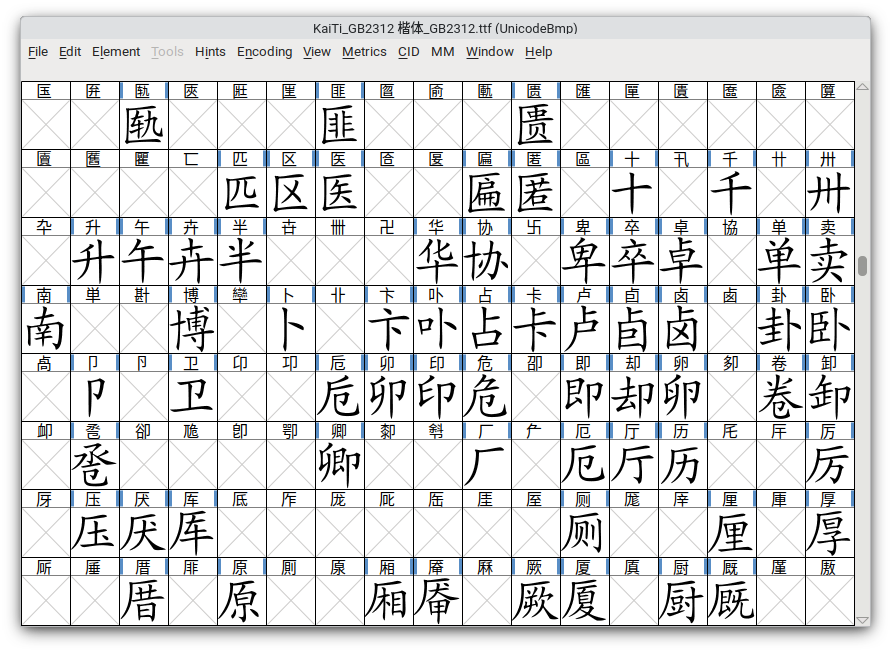
\includegraphics[width=\textwidth]{KaiTi_GB2312 in fontforge.png}
	\caption{\content{在FontForge中打開楷體\_GB2312}{在FontForge中打开楷体\_GB2312}}
	\label{figure:在FontForge中打開楷體GB2312}
\end{figure}
\content{一款字型中有哪些字的字形,這是字型設計者說了算的。中文漢字有十萬餘,其中常用字不過幾千個,所以絕大部分的字型設計者不會把這十萬多字形逐個繪製出來,只會挑選一些可能會用到的字。此外,台灣的字型廠商不太可能去繪製簡體字的字形;大陸的字型廠商也未必會去繪製繁體字的字形。種種因素都會使得中文字型界始終面臨缺字問題的困擾——要輸入生僻人名時,字型顯示不出這個字;要在網路上檢索古籍字時,因為字形不顯示,怎麼也找不到這個字;繁中用戶和簡中用戶交流時,因為使用兩種互不支援的字型,而看不清對方發送的內容——本書作為《繁簡字轉換手冊》,當然有義務幫讀者解決這一問題。}{一款字型中有哪些字的字形,这是字型设计者说了算的。中文汉字有十万余,其中常用字不过几千个,所以绝大部分的字型设计者不会把这十万多字形逐个绘制出来,只会挑选一些可能会用到的字。此外,台湾的字型厂商不太可能去绘制简体字的字形;大陆的字型厂商也未必会去绘制繁体字的字形。种种因素都会使得中文字型界始终面临缺字问题的困扰——要输入生僻人名时,字型显示不出这个字;要在网络上检索古藉字时,因为字形不显示,怎么也找不到这个字;繁中用户和简中用户交流时,因为使用两种互不支持的字形,而看不清对方发送的内容——本书作为《繁简字转换手册》,当然有义务帮读者解决这一问题。}\par
\content{解決字型缺字問題最直接的方法,當然是使用「幾乎不缺字」的字型。「思源」系列的字型就是這方面的典範,它包含六萬餘漢字字形,涵蓋了各地的字形標準,在絕大多數情況下已經可以做到不缺字了。之後又有不少人在思源字型的基礎上加以再創作,製成收字更全的字體,比如遍黑體。除了思源系列的字型以外,坊間還有不少字型也支援大字集,比如來自日本的花園明朝體、來自台灣的全字庫正宋體,以及筆者認為收字最全的「全宋體」,它們多是由志願者自行整理或繪製的。}{解决字型缺字问题最直接的方法,当然是使用“几乎不缺字”的字型。“思源”系列的字型就是这方面的典范,它包含六万余汉字字形,涵盖了各地的字形标准,在绝大多数情况下已经可以做到不缺字了。之后又有不少人在思源字型的基础上加以再创作,制成收字更全的字体,比如遍黑体。除了思源系列的字型以外,坊间还是不少字型也支持大字集,比如来自日本的花园明朝体、来自台湾的全字库正宋体,又及笔者认为收字最全的“全宋体”,它们多是由志愿者自行整理或绘制的。}\par
\content{不過,如果我們希望使用某個收字較少的字型,同時又想盡量避免出現缺字,那麼我們就需要更複雜的排版機制——回落(fallback)字型。簡單說來,我們可以設定一個主字型和一系列回落字型。當排版文字時,優先使用主字型;若是主字型缺字,再依次從回落字型中找這個字,直到找到為止。舉個例子,如果使用思源宋體作為教育部標準楷書體的回落字型,那麼前面的《詩經·小戎》的文段將是這樣的:}{不过,如果我们希望使用某个收字较少的字型,同时又想尽量避免出现缺字,那么我们就需要更复杂的排版机制——回落(fallback)字型。简单说来,我们可以设定一个主字型和一系列回落字型。当排版文字时,优先使用主字型;或是主字型缺字,再依次从回落字型中找到这个字,直到找到为止。举个例子,如果使用思源宋体作为楷体\_GB2312的回落字型,那么前面的《诗经·小戎》的文段将是这样的:}\par
\begin{tcolorbox}[
	natural height,
	enhanced,
	title={——\content{《詩經·小戎》}{《诗经·小戎》}},
	colbacktitle=aa2300,
	attach boxed title to bottom right={xshift=-4mm,yshift=2mm},
	boxed title style={colframe=aa2300},
	colframe=gray!75,
	leftrule=0pt,
	rightrule=0pt,
	sharpish corners,
	leftright skip=1.2em,
	interior style tile={width=\linewidth}{typeset/background.jpg},
]
	\content{\TWMOEStdKai 俴駟孔羣、厹矛鋈錞、蒙伐有苑、虎韔鏤膺、交韔二弓、竹閉緄縢。}{\KaiTiGB2312 俴驷孔群,厹矛鋈錞。蒙伐有苑,虎韔镂膺。交韔二弓,竹闭绲滕。}
\end{tcolorbox}
\content{這樣一來,雖說字體風格不太一致,但我們起碼可以做到讓文字正常顯示了,總比缺字要好。}{这样一来,虽说字体风格不太一致,但我们起码可以做到让文字正常显示了,总比缺字要好。}\par
\subsection{\content{中文編碼}{中文编码}}\label{subsection:中文編碼}
